\documentclass[preprint,12pt]{elsarticle}

\usepackage{amssymb}
\usepackage{amsmath}
\usepackage{graphicx}
\usepackage{booktabs}
\usepackage{algorithm}
\usepackage{algorithmic}
\usepackage{url}
\usepackage{xurl}
\usepackage{array}
\usepackage{float}
\usepackage{placeins}
\usepackage{microtype}
\newcolumntype{L}[1]{>{\raggedright\arraybackslash}p{#1}}
\Urlmuskip=0mu plus 2mu
\emergencystretch=3em

\journal{Applied Soft Computing}

\begin{document}

\begin{frontmatter}

\title{Formula-Inspired Team-Based Evolutionary Optimization with Reactive Redeployment\\ for Dynamic Multi-Objective Tracking}

\author{Ercan Erkalkan\corref{cor1}}
\cortext[cor1]{Corresponding author.}
\ead{ercan.erkalkan@marmara.edu.tr}
\affiliation{
  organization={Department of Computer Technologies, Marmara University},
  addressline={Istanbul},
  country={Turkey}
}

\begin{abstract}
Dynamic multi-objective optimization requires rapid recovery after environmental change under transparent and comparable budgets. However, change-response mechanisms such as redeployment, prediction, and restart policies can create unequal objective-evaluation counts when algorithms are compared only under a common generation horizon. This paper presents Formula-Inspired Team Optimization (FITO), a reactive multi-objective evolutionary algorithm formulated as a DE-inspired bipartite team-guided evolutionary architecture with asymmetric elitism, leader-support coordination, predictive leader anchors, stagnation-triggered local random restart, and post-change redeployment guided by recent leader motion. The main empirical evidence is therefore based on an approximately fixed objective-evaluation budget rather than on a generation-matched protocol. Across DF1--DF9, three dynamic protocols, and 20 independent runs per condition, the primary fixed-budget study calibrates protocol-specific population sizes to approximately 8000 objective evaluations. Under this evaluation-balanced setting, FITO obtains the best overall average MIGD rank (1.898), ahead of NSGA-II (2.711), MDDM-DMOEA (3.415), PPS-DMOEA (4.435), DNSGA-II-A (4.878), DNSGA-II-B (5.280), and KGB-DMOEA (5.383). Holm-corrected pairwise tests in the primary fixed-budget suite give 131 significant FITO wins, 12 significant losses, and 19 non-significant comparisons. A dedicated failure-mode analysis attributes the systematic DF2 losses to a moving decision-variable ownership pattern that invalidates recent leader-motion transfer, and the selected DF7 losses to a time-dependent logistic decision-space linkage that can preserve a smooth objective front while changing the associated decision manifold. A generation-matched 100-population suite is retained only as an auxiliary diagnostic comparison because FITO performs approximately 12,204 objective evaluations on average, whereas the baselines range from 6000 to approximately 7492 evaluations. The auxiliary diagnostic suite shows the same first-rank pattern, but it is not used as the primary fairness claim. Ablations support leader-support coordination, redeployment, predictive anchors, and pit-stop restart, while rejecting boundary-risk scaling and anchor-leader blending. The walk-forward portfolio suite is retained only as a secondary application stress test: the reported tables show a split outcome, with MDDM-DMOEA leading the main MHV summaries in both universes, MDDM-DMOEA or DNSGA-II-A leading MIGD depending on the universe, FITO leading final wealth only in the 14-asset technology universe, and NSGA-II leading final wealth in the broader 20-asset market universe. Consequently, FITO is positioned as a competitive budget-aware dynamic tracking method rather than a universally dominant optimizer or a general finance method.
\end{abstract}

%%Graphical abstract
\begin{graphicalabstract}
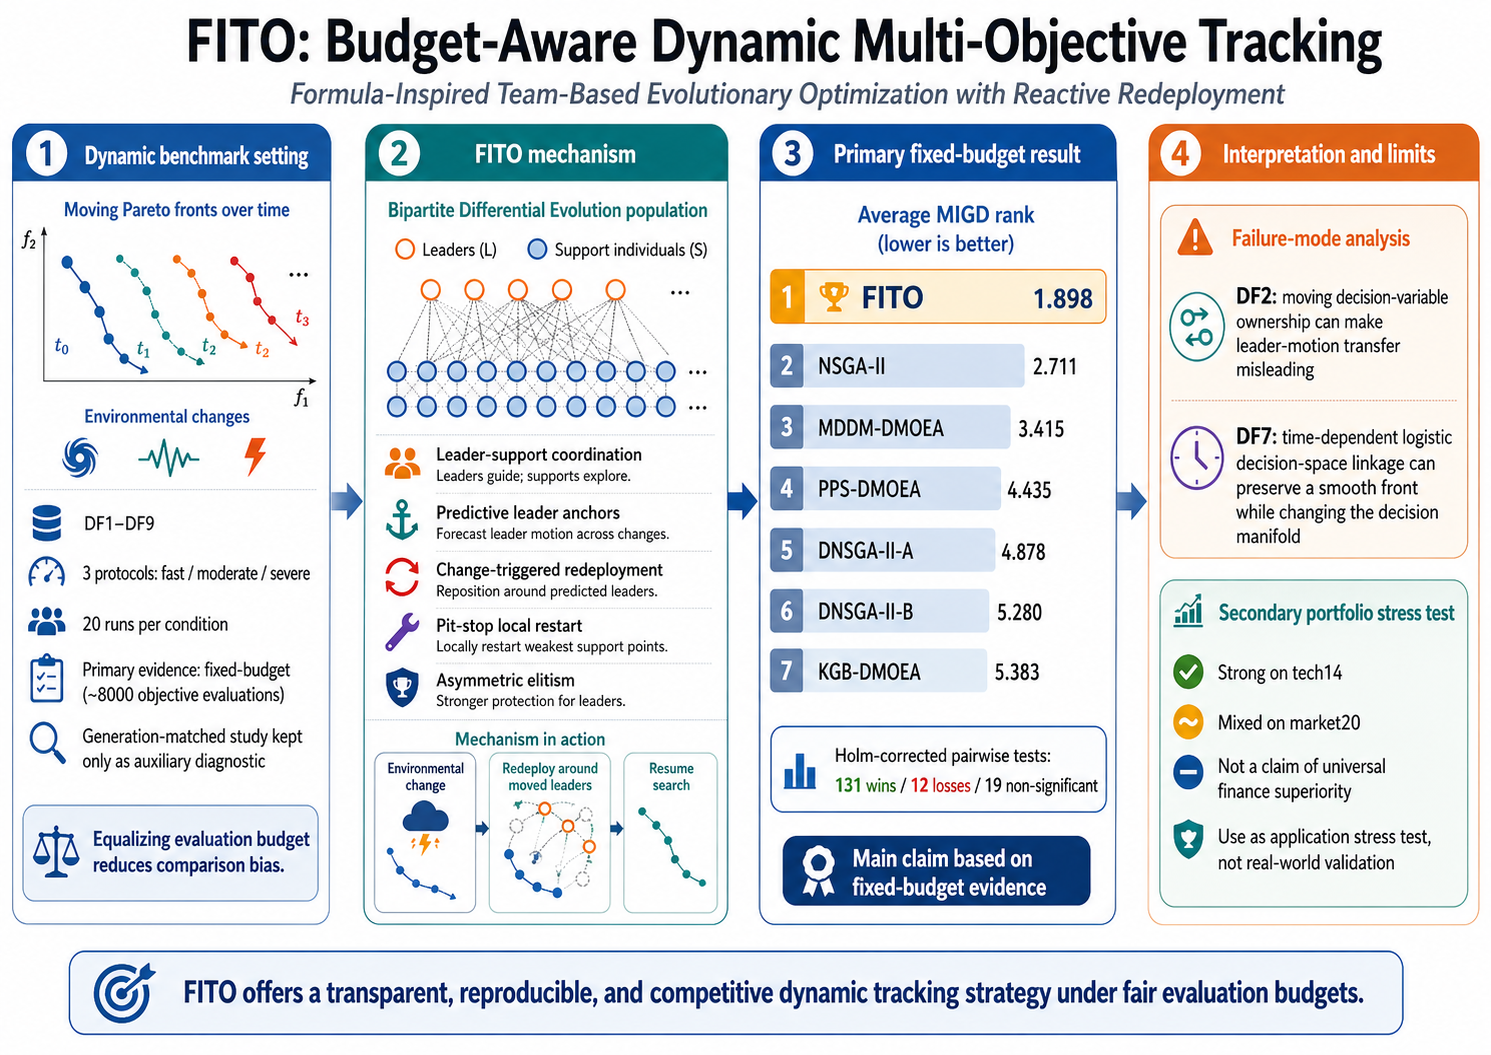
\includegraphics[width=\textwidth]{graphical_abstract.png}
\end{graphicalabstract}

%%Research highlights
\begin{highlights}
\item FITO enables reactive dynamic multi-objective tracking via DE-inspired bipartite search.
\item Fixed-budget DF1--DF9 tests show FITO ranks first by average MIGD.
\item Leader-support coordination, redeployment, and pit-stop restart are validated.
\item DF2/DF7 failure modes reveal limits of leader-motion transfer.
\item Portfolio experiments are framed as a secondary walk-forward stress test.
\end{highlights}

\begin{keyword}
Dynamic multi-objective optimization \sep evolutionary computation \sep restart strategy \sep Pareto tracking \sep benchmark design \sep walk-forward portfolio optimization
\end{keyword}

\end{frontmatter}

\section{Introduction}
\label{sec:introduction}

Many engineering and decision-support problems are intrinsically dynamic. Scheduling, routing, resource dispatch, adaptive control, and online planning are often exposed to changes in objectives, constraints, or operating conditions while optimization is still in progress. In such settings, a useful optimizer must do more than converge to a static Pareto front. It must repeatedly recover after environmental changes and re-establish a high-quality approximation of the moving trade-off surface \cite{Farina2004Dynamic,Gee2017Benchmark}.

Classical multi-objective evolutionary algorithms, including NSGA-II \cite{Deb2002NSGAII}, MOEA/D \cite{Zhang2007MOEAD}, and RVEA \cite{Cheng2016RVEA}, provide strong convergence-diversity mechanisms in static problems. For dynamic settings, several extensions rely on explicit change response or prediction. DNSGA-II introduced change-triggered diversity injection into the NSGA-II framework \cite{Deb2007DNSGAII}. More recent methods exploit historical knowledge more aggressively, for example through Bayesian classification \cite{Ye2022KGB} or predictive population estimation \cite{Gao2024MDDM}. These studies show that dynamic response quality is tightly linked to how an algorithm reuses past information while still preserving enough flexibility to avoid negative transfer.

This study explores a reactive design inspired by Formula 1 team strategy. While the conceptual framing draws from motor racing, the core architecture is mathematically grounded as a DE-inspired bipartite team-guided evolutionary architecture with asymmetric elitism and local random restart. Instead of learning an external predictive model of the next environment, FITO relies on an asymmetric bipartite population (leader-support) structure. This structure modifies traditional elitism by using the elite set not just for preservation, but as active spatial anchors for a directed variant of the DE/current-to-best/1 mutation strategy. Furthermore, the framework incorporates a targeted local random restart (conceptually a pit-stop restart) after internal stagnation, and post-change redeployment informed by recent leader motion. Component testing is used to prune the design: boundary-risk step scaling and anchor-leader blending are retained only if they improve the evidence, and in the final reported method they are rejected.

The main contributions are:
\begin{itemize}
    \item A dynamic MOEA architecture formalized as a DE-inspired bipartite leader-support search process that combines an implementation-level directed differential variation term, stagnation-triggered local random restart (pit-stop), and change-triggered redeployment with predictive leader anchors.
    \item A broader dynamic benchmark design covering DF1--DF9 under three change protocols, 20 independent runs, a primary fixed-budget study, an auxiliary generation-matched diagnostic study, Holm-corrected pairwise testing, and reported effect sizes.
    \item A one-at-a-time component ablation showing that leader-support coordination, redeployment, and pit-stop restart are useful under the expanded protocols, while boundary-risk scaling and anchor-leader blending should be excluded from the default.
    \item A failure-mode analysis of DF2 and DF7 showing where leader-motion transfer can become negative transfer and where local pit-stop restart is insufficient.
    \item A secondary two-universe walk-forward portfolio stress test with three decision rules, three transaction-cost settings, and deterministic equal-weight and rolling-minimum-variance references, used only as an application case study rather than as a real-world validation claim or a claim of general financial superiority.
\end{itemize}

\section{Related work}
\label{sec:related}

Dynamic multi-objective optimization (DMOO) extends static multi-objective evolutionary optimization to environments in which objective functions, constraints, Pareto-optimal sets, or Pareto fronts vary over time. The core difficulty is therefore not only convergence and diversity preservation, but also repeated recovery after environmental change. Recent surveys emphasize that competitive DMOEAs must balance four coupled requirements: detecting or anticipating environmental change, transferring useful historical information without negative transfer, restoring diversity when the search stagnates, and evaluating tracking quality under protocols that do not hide budget or benchmark bias \cite{Azzouz2017Survey,Jiang2022Survey,Shao2026Benchmark}. This section expands the positioning of FITO along these axes.

\subsection{Prediction-based response strategies}

Prediction-based DMOEAs aim to estimate promising search regions after an environmental change and thereby reduce the recovery time needed to track the new Pareto-optimal set. The population prediction strategy (PPS) is a canonical example: historical population displacement is used to initialize a new population that approximates the next environment before ordinary evolutionary search resumes \cite{Zhou2014Population}. Later work refined this idea by predicting representative points, knee points, center points, or multidirectional movements rather than moving the whole population uniformly \cite{Rong2020Multi,Wu2023DSSP,Gao2024CenterMultiDirection,Gao2024MDDM}. The 2024 MOEA/D-MDDM framework is especially relevant because it uses a multidirectional difference model assisted by Pareto-optimal-solution estimation to form a predictive initial population for the new environment \cite{Gao2024MDDM}. Decision-variable-aware prediction has also become increasingly important: DVC-type methods classify decision variables according to their contribution to diversity and convergence, then apply different response policies after change \cite{Liu2021Heterogeneous,Wu2023DVC}.

The benefit of prediction is fast post-change convergence, but the risk is systematic negative transfer. If the Pareto-optimal set changes in a way that invalidates the historical direction, an aggressive predictor can move the population away from the new high-quality region. This risk is central to the DF2 and DF7 behavior observed later in this study. FITO deliberately uses only a short-horizon predictive signal: the most recent displacement of the leader set. This design is less expressive than full population or model-based prediction, but it avoids committing the whole population to a learned global model whose assumptions may be invalid under abrupt topology changes.

\subsection{Transfer learning, memory, and historical reuse}

A second line of work reuses past search information through explicit archives, memory states, or transfer-learning modules. Memory-based approaches store previously useful solutions and retrieve them when similar environments recur, while state-based memory and diversity-maintenance strategies attempt to preserve alternative search directions for future changes \cite{Zou2021Stagnation}. Transfer-learning DMOEAs go further by mapping knowledge from previous source domains to the current target environment. Tr-DMOEA introduced transfer learning into DMOO by constructing a source-target relation across environments \cite{Jiang2018TrDMOEA}. Subsequent knowledge-guided methods include Bayesian classification over historical Pareto-set information \cite{Ye2022KGB}, transfer and maintenance mechanisms for evolving environments \cite{Lin2024KTMO}, and recent twin-population or historical-evolutionary-learning frameworks that use multiple knowledge sources to generate the initial population after change \cite{Zhao2025TMKT,Guan2026EHEL}.

These methods show that historical reuse can be powerful when environments are related, but they also expose the negative-transfer problem. Several recent transfer-based papers explicitly discuss the need to reduce harmful transfer when the source environment is not sufficiently aligned with the target environment \cite{Jiang2018TrDMOEA,Li2025DST}. FITO is positioned as a lightweight alternative to heavy transfer learning: it does not train a domain adapter, density estimator, or cross-environment mapping. Instead, it performs local redeployment around current leaders and short-term predictive anchors. This makes the method simpler and reproducible, but it also explains the observed limitations on DF2 and DF7, where the decision-space relation changes faster than the leader-motion assumption can track.

\subsection{Restart, diversity injection, and stagnation recovery}

Diversity-injection methods remain a foundational response family. DNSGA-II introduced change-triggered replacement of part of the population by random or mutated individuals, giving the search a simple but robust way to re-expand after environmental change \cite{Deb2007DNSGAII}. More recent response frameworks adapt the intensity or type of response according to the estimated environmental change, for example by combining saved historical information, different response operators, or double-space detection in decision and objective spaces \cite{Hu2024HSS,Ma2024DSDRS,Li2024RSAS}. Stagnation recovery is closely related but not identical: an algorithm may stagnate even without an external change. Dual-population and restart-oriented designs address this problem by keeping multiple search components or injecting diversity when progress stops \cite{Li2022Restart}.

FITO's pit-stop restart belongs to this restart/diversity-injection family, but with a narrower scope. Rather than restarting the whole population, only the weakest support individuals are regenerated while the leader set is preserved. This choice is intended to retain the current Pareto-front approximation while freeing local search capacity. The ablation results support this local restart under the tested DF protocols. However, the restart is not a complete safeguard against topology-dependent negative transfer: when active decision-variable roles switch, as in DF2, preserving leaders and perturbing nearby support points can still remain too local.

\subsection{Benchmark protocols, indicators, and fairness of evaluation budgets}

DMOO evaluation is sensitive to benchmark design, change frequency, severity, and performance indicator selection. Classical DF-style and CEC-style benchmarks remain useful because they provide controlled Pareto-set and Pareto-front dynamics \cite{Farina2004Dynamic,Gee2017Benchmark}. Nevertheless, recent benchmarking work argues that next-generation continuous DMOO test suites should include more realistic features such as heterogeneous variable contribution, non-separability, irregular change, and time-linkage effects \cite{Shao2026Benchmark}. This matters because an algorithm that performs well on smooth front motion may fail when the decision manifold changes discontinuously or when historical movement becomes deceptive.

Performance is commonly reported through tracking indicators such as MIGD and hypervolume-based measures. MIGD summarizes the average distance between the obtained approximation and the true time-indexed reference front, while hypervolume provides a convergence-diversity measure based on dominated objective-space volume \cite{Zitzler2000Comparison,Jiang2022Survey}. However, indicator choice alone is insufficient for fair comparison. Dynamic response mechanisms may consume different numbers of objective evaluations even when algorithms are run for the same number of generations. This is particularly important for methods with redeployment, prediction, archive re-evaluation, or change-response operators. For this reason, the present study treats approximately fixed objective-evaluation benchmarking as the primary evidence and retains the generation-matched comparison only as an auxiliary diagnostic.

\subsection{Positioning of FITO relative to recent DMOEA designs}

The recent DMOO literature therefore contains several strong but distinct design philosophies: diversity-injection baselines such as DNSGA-II \cite{Deb2007DNSGAII}, prediction-oriented methods such as PPS, DSSP, DVC, and MDDM \cite{Zhou2014Population,Wu2023DSSP,Wu2023DVC,Gao2024MDDM}, memory and transfer-learning methods such as Tr-DMOEA, KGB-DMOEA, TMKT, and EHEL \cite{Jiang2018TrDMOEA,Ye2022KGB,Zhao2025TMKT,Guan2026EHEL}, adaptive change-response frameworks such as HRS-DMOA, MOEA/D-HSS, DSDRS, and RSAS \cite{Li2024HRS,Hu2024HSS,Ma2024DSDRS,Li2024RSAS}, and restart/stagnation-recovery mechanisms \cite{Li2022Restart,Zou2021Stagnation}. FITO does not claim to dominate all of these families. Its leader-support division also draws on the broader swarm-intelligence idea that different individuals can play different guidance roles, as in particle-swarm coordination, but it implements this idea through a constrained DE-inspired bipartite team-guided topology rather than through velocity attraction \cite{Eberhart1995PSO}. Its contribution is narrower: a transparent, reproducible, budget-aware architecture that combines asymmetric leader-support coordination, short-horizon anchor redeployment, and localized pit-stop restart without requiring a heavy external prediction or transfer model.

This positioning also motivates the baseline policy. Exact reimplementation of recent complex prediction and transfer-learning methods can introduce implementation bias when authoritative code is unavailable. Therefore, the empirical comparison prioritizes reproducible implementations and a fixed-budget fairness layer, while the related-work discussion explicitly situates FITO against recent 2023--2026 developments in prediction, transfer, response adaptation, restart, and benchmarking.

\section{Problem formulation}
\label{sec:problem}

A dynamic multi-objective minimization problem is considered
\begin{equation}
\min_{x \in \Omega} \; F(x,t) = \left(f_1(x,t), f_2(x,t), \ldots, f_m(x,t)\right),
\end{equation}
where $\Omega \subseteq \mathbb{R}^{n}$ denotes the feasible decision space and $t$ denotes the current environment. Both the Pareto-optimal set and Pareto front may vary with time.

For dynamic problems, the main performance indicator is mean inverted generational distance (MIGD),
\begin{equation}
\mathrm{MIGD} = \frac{1}{T}\sum_{t=1}^{T}\mathrm{IGD}\left(P_t^{\mathrm{approx}}, P_t^\star\right),
\end{equation}
where $P_t^{\mathrm{approx}}$ is the approximated non-dominated set and $P_t^\star$ is the true Pareto front at environment $t$. Smaller MIGD values indicate better overall tracking behavior.

For the static sanity check, hypervolume (HV) and IGD are used on ZDT benchmarks \cite{Zitzler2000Comparison}.

\section{Formula-Inspired Team Optimization}
\label{sec:method}

\subsection{Leader-support population structure}

At generation $g$, the population is ranked by non-dominated sorting and crowding distance. The top
\begin{equation}
n_L = \max(6,\lfloor 0.1N \rfloor)
\end{equation}
solutions form the leader set $\mathcal{L}_g$, and the remaining solutions form the support pool. Leaders provide directional guidance, while support individuals preserve maneuverability and absorb restart operations.

Offspring are generated by simulated binary crossover, polynomial mutation, and a two-child team-guided correction that matches the released implementation. After parent selection and SBX, the two children $c_1$ and $c_2$ are updated asymmetrically as
\begin{align}
c_1' &= \Pi_{[x_l,x_u]}\left(c_1 + \lambda_1(x_L-c_1)\right), \\
c_2' &= \Pi_{[x_l,x_u]}\left(c_2 + \lambda_2(x_a-x_b)\right),
\label{eq:update}
\end{align}
where $x_L \in \mathcal{L}_g$ is a sampled leader, $x_a-x_b$ is a differential diversity term sampled from the current population, $\Pi_{[x_l,x_u]}(\cdot)$ denotes clipping to the feasible decision bounds, $\lambda_1=0.10$, and $\lambda_2=0.15$. Thus, the leader-pull term is applied to $c_1$, whereas the differential-push term is applied to $c_2$; the two terms are not summed on a single offspring vector. These directional and differential scaling multipliers were established through a preliminary empirical grid search targeting stable Pareto-tracking performance (see Section~\ref{subsec:sensitivity} for the sensitivity analysis of $\lambda_1$). Leader-guided pairings are used with probability 0.8; otherwise, parents are selected by tournament on dominance rank and crowding distance.

It is critical to formally position this variation strategy as a two-child directed variant of DE/current-to-best-style search, adapted for a bipartite population. In classical elitism, top-ranked solutions are passively preserved into the next generation. In FITO's asymmetric elitism, the leader set $\mathcal{L}_g$ acts actively as directional anchors for one child, while the second child receives a separate differential diversity displacement. Eq.~(\ref{eq:update}) therefore does not describe a generic single-vector DE/current-to-best/1 mutation. Instead, it describes the implementation-level asymmetric offspring update: $c_1$ is pulled toward a sampled leader from $\mathcal{L}_g$, and $c_2$ is moved by an independent differential vector $x_a-x_b$. Consequently, the operator combines directed leader exploitation and diversity-preserving differential exploration without applying both corrections to the same child.
\subsection{Pruned variants and ablation strategy}

During the algorithm design, various mechanisms were tested, and those that did not provide a performance increase were eliminated. The formal analysis of these eliminated features is presented in Section~\ref{sec:results}. One such feature was a boundary-risk multiplier intended to scale the team-guided correction near the feasible-space boundaries. The FITO+BR variant tests the inclusion of this multiplier:
\begin{equation}
r(x) = \mathrm{clip}\left(0.35 + 1.3 \cdot \frac{1}{n}\sum_{i=1}^{n}\min(\tilde{x}_i, 1-\tilde{x}_i),\,0.35,\,1.0\right),
\label{eq:risk}
\end{equation}
where
\begin{equation}
\tilde{x}_i = \frac{x_i-l_i}{u_i-l_i},
\end{equation}
and $l_i$ and $u_i$ are the lower and upper bounds of the $i$-th variable. FITO+BR replaces both correction terms in Eq.~(\ref{eq:update}) by $r(x)$-scaled terms. Because it did not improve overall performance, the final FITO default does not use this scaling.

\subsection{Default stagnation restart and reactive redeployment}

FITO includes one default-enabled stagnation-triggered pit-stop restart branch and one active change-triggered redeployment mechanism. The restart branch is optional only in the ablation setting that disables pit-stop behavior; it is active in the final FITO default used in the main experiments. To avoid any dependence on external benchmark information, stagnation is detected with an internal quality score based only on the current non-dominated set:
\begin{equation}
q_g = \mathrm{HV}\left(\hat{P}^{ND}_g; \mathbf{r}\right),
\end{equation}
where $\hat{P}^{ND}_g$ is the current non-dominated set normalized by the current population ideal and nadir vectors, and $\mathbf{r}=(1.1,\ldots,1.1)$ is the reference point. If $q_g$ has not improved for $s=8$ generations (the stagnation tolerance, established via preliminary sensitivity analysis in Section~\ref{subsec:sensitivity}), the weakest
\begin{equation}
n_R = \max(4,\lfloor 0.125N \rfloor)
\end{equation}
support individuals are replaced either by Gaussian perturbations around randomly sampled leaders or by opposition-style reflections. The perturbation scale is set to $\sigma = 0.08$ of the decision-space width, and the replacement fraction $0.125N$ ensures a local rather than global reset.

Unlike standard stagnation-based restart mechanisms that often reinitialize the entire population or apply uniformly distributed diversity injections, this local random restart (conceptually framed as a ``pit-stop'') is a highly localized, partial reset. It keeps the high-performing leader set strictly intact to preserve the accumulated approximation of the Pareto surface. By targeting only the weakest portion of the support pool and regenerating them in the immediate vicinity of the current leaders, the method avoids catastrophic forgetting while rapidly re-establishing search momentum in regions with the highest probability of yielding improvements.

The second mechanism is change-triggered redeployment. After an environmental change, FITO immediately re-evaluates the retained population and repositions the weakest
\begin{equation}
n_C = \max(4,\lfloor 0.08N \rfloor)
\end{equation}
support individuals around the current leader set. In both cases, weakness is defined within the support pool by higher non-dominated rank first and, among ties, lower crowding distance. The $0.08N$ redeployment fraction was selected empirically to provide sufficient reaction mass without overriding the entire support pool. This is the active post-change redeployment response in the main dynamic benchmark.

Redeployment is partly informed by recent leader drift. Let $\mathcal{L}^{\mathrm{pre}}_{t-1}$ and $\mathcal{L}^{\mathrm{pre}}_{t}$ denote the leader sets immediately before two consecutive environmental changes, and let $\bar{\ell}_{t-1}$ and $\bar{\ell}_{t}$ be their centroids. When both are available, FITO forms a predictive anchor pool
\begin{equation}
\mathcal{A}_{t} = \mathrm{clip}\left(\mathcal{L}^{\mathrm{pre}}_{t} + (\bar{\ell}_{t} - \bar{\ell}_{t-1}),\, \mathbf{l},\, \mathbf{u}\right),
\end{equation}
which is a one-step extrapolation of the most recent leader motion. Here, the $\mathrm{clip}(\cdot, \mathbf{l}, \mathbf{u})$ function enforces the lower bounds $\mathbf{l}$ and upper bounds $\mathbf{u}$ of the decision space by projecting any out-of-bound variables back to their respective boundaries. For the first $\lceil 0.5 n_C \rceil$ redeployed support individuals, the final FITO default uses a sampled anchor $a \in \mathcal{A}_{t}$ directly as the redeployment base. Another evaluated feature was anchor-leader blending, which combines an anchor with a current leader $\ell \in \mathcal{L}_{t}$ as:
\begin{equation}
b = 0.65\, a + 0.35\, \ell.
\end{equation}
Because the ablation study identifies this blend as non-beneficial, it is excluded from the default design and reported only as the FITO+MB variant in Section~\ref{sec:results}. The remaining redeployments use current leaders only. Anchor-based redeployments use Gaussian perturbations with scale $0.35\sigma$, whereas leader-only redeployments use $0.6\sigma$. Figure~\ref{fig:redeployment_concept} conceptually illustrates this change-triggered redeployment mechanism in the decision space.

\begin{figure}[!t]
\centering
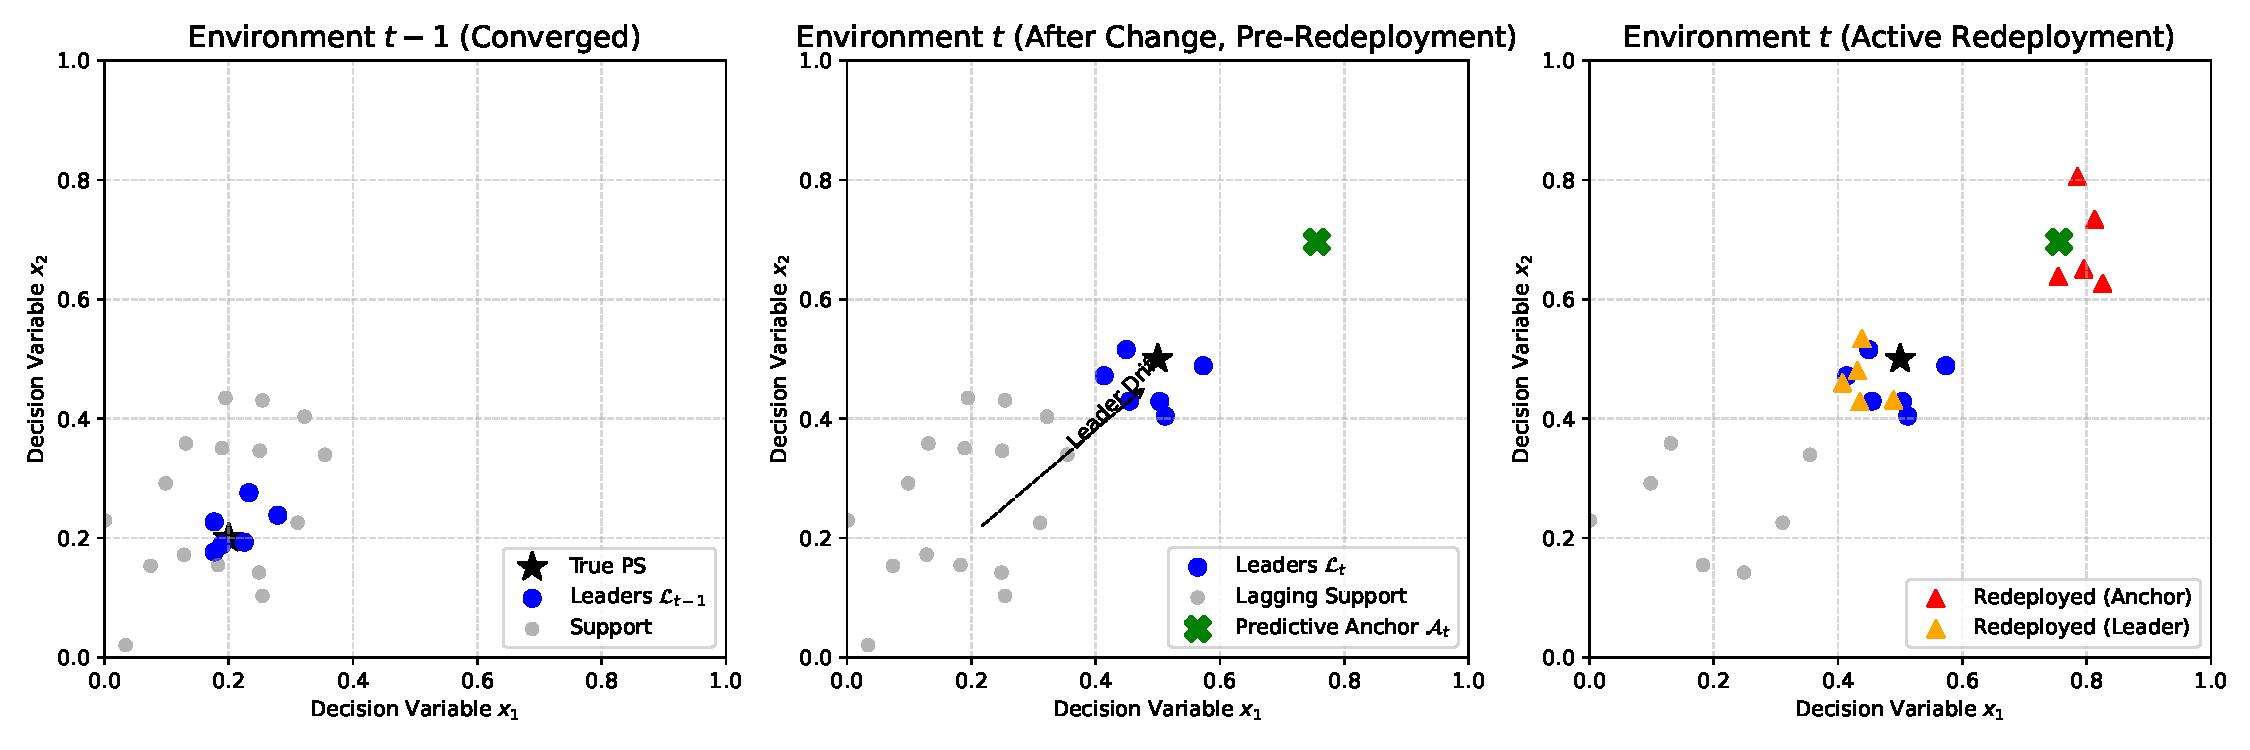
\includegraphics[width=\textwidth]{../experiments/results/redeployment_concept.pdf}
\caption{Conceptual 2D illustration of the change-triggered redeployment mechanism. At environment $t-1$, the population is converged. After an environmental change to $t$, the leader set $\mathcal{L}_t$ successfully tracks the new front, but support individuals lag behind. FITO computes a predictive anchor $\mathcal{A}_t$ based on the collective drift and actively redeploys the weakest lagging support individuals around the new anchors and current leaders, accelerating recovery.}
\label{fig:redeployment_concept}
\end{figure}

\subsection{Algorithmic flow}

Algorithm~\ref{alg:fito} summarizes the complete procedure and explicitly lists the implementation-level restart and redeployment decisions used by the released code. The baseline generational complexity is dominated by non-dominated sorting, giving $O(mN^2)$ for selection plus $O(Nn)$ for variation. However, unlike standard NSGA-II, FITO computes the hypervolume of the normalized non-dominated set $\hat{P}^{ND}_g$ at every generation to monitor stagnation ($q_g$). While exact hypervolume calculation is $O(N \log N)$ for $m=2$ objectives and has representative higher-dimensional bounds such as $O(N \log N + N^{m/2})$ or $O(N^{m-2} \log N)$ for $m \ge 3$, it becomes rapidly more expensive as the number of objectives increases. For the 2-objective benchmark and portfolio problems studied here, this internal HV calculation is computationally trivial and does not alter the overall $O(N^2)$ generational complexity. For many-objective extensions ($m > 3$), exact per-generation HV calculation may become a severe computational bottleneck, necessitating either a switch to an approximation method (e.g., Monte Carlo sampling) or a substitution of the stagnation metric with a cheaper alternative like IGD against a reference set or a generational distance-based metric.

\begin{algorithm}[!t]
\footnotesize
\caption{Formula-Inspired Team Optimization (FITO)}
\label{alg:fito}
\begin{algorithmic}[1]
\REQUIRE Population size $N$, generations $G$, stagnation tolerance $s=8$
\STATE Set $n_L=\max(6,\lfloor0.1N\rfloor)$, $n_R=\max(4,\lfloor0.125N\rfloor)$, $n_C=\max(4,\lfloor0.08N\rfloor)$, and restart scale $\sigma=0.08$
\STATE Initialize population uniformly in the feasible space and evaluate objective vectors
\FOR{$g=1$ to $G$}
    \STATE Rank the population by non-dominated sorting and crowding distance
    \STATE Form leader set $\mathcal{L}_g$ with $n_L$ solutions and define the remaining population as support
    \STATE Generate offspring using leader-support mating, SBX crossover, the two-child correction in Eq.~(\ref{eq:update}), and polynomial mutation
    \STATE Merge parents and offspring and keep the best $N$ solutions
    \STATE Update the normalized non-dominated-set quality score $q_g$
    \IF{no improvement in $q_g$ is observed for $s$ generations}
        \STATE Select the weakest $n_R$ support individuals by rank and crowding distance
        \STATE Replace them by leader-centred Gaussian perturbations or opposition-style reflections while preserving all leaders
    \ENDIF
    \IF{the environment changes}
        \STATE Re-evaluate the retained population and update the current leader set $\mathcal{L}_t$
        \STATE Select the weakest $n_C$ support individuals by rank and crowding distance
        \IF{pre-change leader centroids from two consecutive changes are available}
            \STATE Build the predictive anchor pool $\mathcal{A}_t=\mathrm{clip}(\mathcal{L}^{\mathrm{pre}}_t+(\bar{\ell}_t-\bar{\ell}_{t-1}),\mathbf{l},\mathbf{u})$
            \STATE Redeploy the first $\lceil0.5n_C\rceil$ selected supports around sampled anchors using Gaussian scale $0.35\sigma$
            \STATE In FITO+MB only, replace each anchor base by $0.65a+0.35\ell$; default FITO uses anchors without blending
        \ENDIF
        \STATE Redeploy all remaining selected supports around sampled current leaders using Gaussian scale $0.6\sigma$
    \ENDIF
\ENDFOR
\STATE \textbf{return} the non-dominated approximation set
\end{algorithmic}
\end{algorithm}

\section{Experimental design}
\label{sec:experiments}

\subsection{Implementation}

All experiments were implemented in Python 3.14 with \texttt{pymoo} 0.6.1.6 \cite{Blank2020Pymoo}. Market-data acquisition for the broader portfolio universe was handled through locally cached \texttt{yfinance} downloads. FITO was implemented from scratch. The repository includes the experiment scripts, cached data files, generated tables, and the manuscript source; \texttt{reproduce\_all.ps1} reruns the full pipeline from the repository root.

\subsection{Dynamic benchmarks and baselines}

The primary synthetic study uses all nine two-objective DF instances, DF1--DF9. Three environment-change protocols are evaluated over a 60-generation horizon: a fast protocol with \texttt{taut}=5 and \texttt{nt}=10, a moderate protocol with \texttt{taut}=10 and \texttt{nt}=10, and a more severe protocol with \texttt{taut}=10 and \texttt{nt}=20. The auxiliary generation-matched diagnostic uses a common population size of 100, whereas the primary fixed-budget study uses protocol- and algorithm-specific calibrated population sizes to approximate the target nominal evaluation budget. This produces 27 protocol-problem cases and tests both frequent and slower environmental changes.

Six baselines are used in the dynamic comparison:
\begin{itemize}
    \item DNSGA-II-A \cite{Deb2007DNSGAII}
    \item DNSGA-II-B \cite{Deb2007DNSGAII}
    \item KGB-DMOEA \cite{Ye2022KGB}
    \item MDDM-DMOEA \cite{Gao2024MDDM}
    \item NSGA-II \cite{Deb2002NSGAII}
    \item PPS-DMOEA \cite{Zhou2014Population}
\end{itemize}

The selection of baselines intentionally prioritizes algorithms with verified, reproducible public implementations. Recent DMOO research includes prediction-based, decision-variable-aware, historical-memory, transfer-learning, and adaptive-response designs such as DSSP, DVC, MDDM, HRS-DMOA, MOEA/D-HSS, DSDRS, RSAS, TMKT, and EHEL \cite{Wu2023DSSP,Wu2023DVC,Gao2024MDDM,Li2024HRS,Hu2024HSS,Ma2024DSDRS,Li2024RSAS,Zhao2025TMKT,Guan2026EHEL}. Reimplementing all of these complex methods from descriptions alone would create substantial implementation bias. Therefore, the benchmark uses reproducible representatives that cover the major response families: DNSGA-II variants for diversity injection, PPS-DMOEA for population prediction, KGB-DMOEA for knowledge-guided Bayesian transfer, MDDM-DMOEA through an open-source KDE-based surrogate of the 2024 multidirectional difference framework, and NSGA-II as a static evolutionary reference.

All dynamic experiments use 20 independent runs with seeds 0--19. The dynamic benchmark is reported in two layers to avoid a misleading fairness interpretation. The primary layer is an approximately fixed-budget protocol that calibrates the population size separately for each algorithm and dynamic protocol to target approximately 8000 objective evaluations while preserving the nominal generation count. The calibration is deliberately lightweight: for each algorithm--protocol pair, the candidate population size is selected from a DF1, seed-0 pilot run and then frozen before the full DF1--DF9, seed-0--19 evaluation is executed. This pilot-based calibration avoids tuning the population size on the full benchmark outcomes, but it also means that the budget target is approximate rather than a multi-problem optimum. Therefore, nominal evaluation means, response-refresh evaluation means, total objective-call means, and calibrated population sizes are reported explicitly in Table~\ref{tab:dynamic-fixed-budget}. This layer is used for the main performance claim because dynamic response operators do not consume objective evaluations uniformly across algorithms. The auxiliary layer is a conventional generation-matched diagnostic with a common population size of 100. The auxiliary layer is retained for interpretability and comparison with standard dynamic evolutionary benchmarking practice, but it is not used as the primary evidence of algorithmic superiority. In the auxiliary layer, FITO performs approximately 12,204 nominal objective evaluations on average because redeployment and response operations add evaluations, whereas the baselines range from 6000 nominal evaluations for NSGA-II, MDDM-DMOEA, and PPS-DMOEA to approximately 7190--7943 nominal evaluations for DNSGA-II and KGB-DMOEA variants. For MDDM-DMOEA and PPS-DMOEA, additional predictive response refreshes are also reported separately as \texttt{response\_evaluation\_count}; therefore, nominal and total objective-call counts are not silently conflated. This separation prevents the central conclusion from depending on an unequal-evaluation generation-matched comparison. Statistical comparisons use two-sided Mann--Whitney $U$ tests with Holm correction, and Cliff's $\delta$ effect sizes and 95\% confidence intervals for the mean are additionally reported. The one-at-a-time ablation uses FITO-noLS, FITO-noRD, FITO-noPA, FITO-noPS, FITO+BR, and FITO+MB. FITO-noPS disables only the pit-stop restart while keeping redeployment active.

\subsection{Static sanity check}

To assess whether the implementation remains reasonable outside the dynamic setting, FITO is also evaluated on ZDT1, ZDT2, ZDT3, ZDT4, and ZDT6 against NSGA-II, MOEA/D, and RVEA. The static run keeps the same internal stagnation score $q_g$ and restart trigger, but the environment does not move and change-triggered redeployment is absent. Static significance tests also use Mann--Whitney $U$ with global Holm correction. These results are supplementary rather than primary evidence for the dynamic claim.

\subsection{Walk-forward portfolio suite}

The application study is expanded into two 38-period walk-forward universes: the original 14-asset technology universe and a broader 20-asset large-cap market universe spanning multiple sectors. The cached price files cover the broader 2012--2022 interval; the generated walk-forward environments use trailing training windows beginning in May 2012 and evaluate unseen holdout windows from 2013-05-23 to 2022-11-22. This subsection is deliberately designed as a secondary application stress test, not as a real-world validation claim and not as evidence that FITO is a generally superior financial optimizer. At each environment, a trailing 252-trading-day window is used to estimate mean returns and covariance, the algorithm optimizes the estimated long-only mean-variance problem for 10 generations, and deployment is evaluated over the next unseen 63-trading-day holdout window. The primary reporting rule selects the non-dominated portfolio closest to the normalized ideal point with turnover as a tie-break, but max-Sharpe and minimum-variance deployment rules, as well as three transaction-cost settings (5, 10, and 25 bps), are also evaluated. Deterministic equal-weight and rolling minimum-variance strategies are added as deployment references. The portfolio suite reports a generation-matched optimization family and a fixed-budget auxiliary study through per-universe population calibration. The auxiliary budget family targets approximately 60,000 nominal training-objective evaluations, but the realized counts differ by algorithm and universe; the raw metrics therefore report realized \texttt{n\_evals} and separate response-refresh counts for audit rather than treating the target as exactly met. Pairwise FITO-versus-baseline tests use two-sided Mann--Whitney $U$ tests with Holm correction within each reported metric family. The holdout reference frontier is approximated by a dense long-only efficient-frontier sweep solved by convex scalarization. Four finance-specific restrictions are kept explicit: the universes are fixed ex post and therefore can still contain survivorship or selection bias; the 2013-05-23--2022-11-22 holdout schedule may favor or penalize particular sector structures; transaction costs are represented by simple proportional bps charges without market impact, liquidity, borrowing, tax, or slippage models; and the efficient-frontier approximation is long-only, excluding shorting, leverage, and cash allocation.

\section{Results and discussion}
\label{sec:results}


\subsection{Primary fixed-budget dynamic benchmark}
\label{subsec:primary-fixed-budget-results}

\begin{table}[!t]
\centering
\caption{Primary fixed-budget average MIGD ranks across dynamic protocols. Lower is better.}
\label{tab:dynamic-budget-ranks}
\resizebox{\textwidth}{!}{%
\begin{tabular}{lccccccc}
\toprule
Protocol & FITO & DNSGA-II-A & DNSGA-II-B & KGB-DMOEA & MDDM-DMOEA & NSGA-II & PPS-DMOEA \\
\midrule
fast\_t5\_n10 & \textbf{2.139} & 4.517 & 5.533 & 5.244 & 3.350 & 2.617 & 4.600 \\
moderate\_t10\_n10 & \textbf{1.678} & 5.033 & 5.439 & 5.000 & 3.611 & 2.594 & 4.644 \\
severe\_t10\_n20 & \textbf{1.878} & 5.083 & 4.867 & 5.906 & 3.283 & 2.922 & 4.061 \\
\midrule
Overall & \textbf{1.898} & 4.878 & 5.280 & 5.383 & 3.415 & 2.711 & 4.435 \\
\bottomrule
\end{tabular}
}
\end{table}


The primary dynamic benchmark uses the approximately fixed objective-evaluation protocol described in Section~\ref{sec:experiments}. Table~\ref{tab:dynamic-fixed-budget} reports the realized nominal evaluation means, response-refresh evaluation means, total objective-call means, and protocol-specific population sizes, and Table~\ref{tab:dynamic-budget-ranks} reports the corresponding average MIGD ranks. The nominal evaluation counts are tightly aligned around the 8000-evaluation target: FITO averages approximately 8052 nominal evaluations across protocols, DNSGA-II-A and DNSGA-II-B average approximately 8044, KGB-DMOEA averages approximately 8015, and MDDM-DMOEA, NSGA-II, and PPS-DMOEA average 7980. The audit also exposes that MDDM-DMOEA and PPS-DMOEA require additional response-refresh evaluations (1596 under the fast protocol and 798 under the moderate and severe protocols). Thus, the fixed-budget claim applies to the nominal optimizer budget, while total objective calls are reported explicitly rather than hidden. The design therefore makes the fixed-budget result the main fairness-controlled comparison, while leaving equal-population behavior to the auxiliary diagnostic study.

Under this primary protocol, FITO achieves the best overall average MIGD rank, with 1.898 across the complete DF1--DF9 benchmark and the three dynamic protocols. The next best method is NSGA-II with an overall average rank of 2.711, followed by MDDM-DMOEA (3.415), PPS-DMOEA (4.435), DNSGA-II-A (4.878), DNSGA-II-B (5.280), and KGB-DMOEA (5.383). FITO ranks first in each protocol-level aggregation: 2.139 under \texttt{fast\_t5\_n10}, 1.678 under \texttt{moderate\_t10\_n10}, and 1.878 under \texttt{severe\_t10\_n20}. Holm-corrected pairwise tests over 162 FITO-versus-baseline comparisons yield 131 significant FITO wins, 12 significant FITO losses, and 19 non-significant comparisons. The main empirical claim is therefore restricted to evaluation-balanced dynamic benchmarking: FITO remains the strongest average-rank method when the objective-evaluation budget is approximately equalized.

The fixed-budget results also delimit the method. Significant losses are concentrated in DF2 and selected DF7 cases, with one additional DF1 loss against NSGA-II under the fast protocol. This pattern indicates that the FITO response stack is not universally dominant. The strongest claim supported by the evidence is not universal superiority on every dynamic landscape, but robust average-rank leadership under a controlled objective-evaluation budget. The two concentrated failure families are analyzed explicitly in Section~\ref{subsec:failure-modes}.

\subsection{Auxiliary generation-matched diagnostic}
\label{subsec:generation-matched-diagnostic}

\begin{table}[!t]
\centering
\caption{Auxiliary generation-matched average MIGD ranks across dynamic protocols. Lower is better.}
\label{tab:dynamic-protocol-ranks}
\resizebox{\textwidth}{!}{%
\begin{tabular}{lccccccc}
\toprule
Protocol & FITO & DNSGA-II-A & DNSGA-II-B & KGB-DMOEA & MDDM-DMOEA & NSGA-II & PPS-DMOEA \\
\midrule
fast\_t5\_n10 & \textbf{1.739} & 4.383 & 5.128 & 5.272 & 3.567 & 2.922 & 4.989 \\
moderate\_t10\_n10 & \textbf{1.422} & 4.617 & 5.211 & 4.806 & 3.956 & 2.950 & 5.039 \\
severe\_t10\_n20 & \textbf{1.500} & 4.728 & 4.594 & 5.728 & 3.744 & 3.211 & 4.494 \\
\midrule
Overall & \textbf{1.554} & 4.576 & 4.978 & 5.269 & 3.756 & 3.028 & 4.841 \\
\bottomrule
\end{tabular}
}
\end{table}


The generation-matched 100-population benchmark is retained as an auxiliary diagnostic rather than as the primary fairness-controlled result. Table~\ref{tab:dynamic-eval-budget} shows why this distinction is necessary. FITO performs approximately 12,204 nominal objective evaluations on average in this setting, whereas DNSGA-II-A and DNSGA-II-B average approximately 7190--7790 evaluations depending on protocol, KGB-DMOEA averages approximately 7266--7943, and MDDM-DMOEA, NSGA-II, and PPS-DMOEA average 6000. The MDDM-DMOEA and PPS-DMOEA response-refresh counts are shown separately, so their total objective-call effort is also auditable. Consequently, the generation-matched comparison evaluates the behavior of full algorithmic pipelines under a common generation schedule, but it does not equalize objective-evaluation effort.

Within this diagnostic setting, Table~\ref{tab:dynamic-protocol-ranks} shows that FITO again obtains the best overall average MIGD rank (1.554), ahead of NSGA-II (3.028), MDDM-DMOEA (3.756), DNSGA-II-A (4.576), PPS-DMOEA (4.841), DNSGA-II-B (4.978), and KGB-DMOEA (5.269). The method remains first in all three protocol aggregates: 1.739 in the fast \texttt{taut}=5 regime, 1.422 in the moderate \texttt{taut}=10 regime, and 1.500 in the severe \texttt{taut}=10, \texttt{nt}=20 regime. Holm-corrected testing over 162 diagnostic FITO-versus-baseline comparisons records 144 significant FITO wins, 10 significant FITO losses, and 8 non-significant comparisons. These results are useful for interpreting the full response behavior of each method under the same generation horizon. Nevertheless, the diagnostic rank of 1.554 is not used as the headline fairness claim because the objective-evaluation counts are unequal. The fixed-budget rank of 1.898 is the appropriate primary result.

The activation audit confirms that MDDM-DMOEA and PPS-DMOEA no longer collapse to NSGA-II: both baselines register nonzero change-response counts, whereas NSGA-II remains the intended zero-response baseline. The extra predictive response refreshes for MDDM-DMOEA and PPS-DMOEA are recorded separately as \texttt{response\_evaluation\_count} rather than being hidden in the nominal evaluation budget. Detailed protocol-specific MIGD tables are reported in the dynamic appendix.

\subsection{Failure-mode analysis on DF2 and DF7}
\label{subsec:failure-modes}

The fixed-budget protocol makes the main losses interpretable because they cannot be dismissed as artifacts of unequal objective-evaluation counts. The losses are not random across the benchmark. DF2 produces systematic FITO losses against NSGA-II, DNSGA-II-A, and KGB-DMOEA in all three protocols. Under the fixed-budget setting, FITO obtains mean MIGD values of 0.2969, 0.2175, and 0.1878 on the fast, moderate, and severe DF2 protocols, respectively. The corresponding NSGA-II values are 0.0970, 0.0973, and 0.0659; DNSGA-II-A obtains 0.1472, 0.1290, and 0.1071; and KGB-DMOEA obtains 0.1904, 0.1306, and 0.1132. These differences remain Holm-significant against the three baselines in all three DF2 protocols.

The structural reason is the special DF2 decision topology. In the DF implementation, the first objective is not tied permanently to a fixed coordinate; instead, the active coordinate index is $r=\lfloor (n-1)|\sin(\pi t/2)| \rfloor$, and $f_1=x_r$ while the remaining coordinates enter the distance term $g$. Thus, environmental change can alter which decision variable carries the Pareto-front parameter. This is not a smooth translation of the same decision manifold. It is a coordinate-role switch. FITO's leader-support and redeployment rules intentionally exploit short-term leader motion, but this assumption becomes fragile when the identity of the objective-driving variable changes. A leader displacement observed before the change may point in a formerly useful coordinate direction. After a DF2 coordinate-role switch, the same transferred displacement can pull support individuals toward the wrong manifold. This explains why leader-support plus redeployment can create negative transfer on DF2 rather than useful acceleration.

The pit-stop restart does not fully repair this failure because it is deliberately local. The restart branch regenerates only a small fraction of weak support individuals while preserving leaders and most population geometry. This design is beneficial when the Pareto set moves smoothly or when only part of the support pool stagnates. DF2 requires a broader reallocation of decision-variable roles. Preserving leaders after a coordinate-role switch can preserve obsolete structural information, and regenerating a limited support subset is too weak to rebuild the population around the newly active coordinate. By contrast, NSGA-II has no explicit leader-motion transfer and no preserved anchor dependency. Its crowding-based survival and generic variation maintain a more neutral spread, which is less efficient on many smooth-tracking problems but more robust on DF2. DNSGA-II-A and KGB-DMOEA also benefit because their response mechanisms inject or infer diversity without committing as strongly to the most recent leader displacement.

DF7 is a different and milder failure mode. FITO is not systematically poor on DF7. In the primary fixed-budget suite, the significant losses are concentrated in the fast protocol: FITO gives 0.2742 mean MIGD, whereas NSGA-II gives 0.1526 and MDDM-DMOEA gives 0.1678. Under the moderate protocol, FITO is close to MDDM-DMOEA and NSGA-II, and the Holm-corrected differences are not significant; under the severe protocol, FITO has the best mean value among the compared methods. The issue is therefore not universal DF7 incompatibility, but sensitivity to rapid changes.

DF7 combines a smooth reciprocal objective front with a nonlinear time-dependent decision-space linkage. The Pareto front is parameterized by $f_1=(1+t)/x_0$ and $f_2=x_0/(1+t)$, but the remaining variables are tied to $x_0$ through a logistic target $1/(1+\exp(a(x_0-2.5)))$, where $a=5\cos(\pi t/2)$. As $t$ changes, the objective front may remain smooth while the decision-space manifold associated with that front changes curvature and orientation. This decouples objective-space regularity from decision-space transferability. FITO's anchors can track the apparent front motion, but the support pool may still carry obsolete $x_0$-conditioned linkage information. Fast DF7 changes leave too little time for the local restart and redeployment operators to correct this mismatch. MDDM-DMOEA's distributional response and NSGA-II's broader population spread are therefore competitive in the fast case.

These failures clarify the intended operating regime of FITO. The method is strongest when recent leader motion is a reliable proxy for the next useful search region, as in recurring, sector-like, or topologically stable drift. The method is weaker when environmental change modifies the identity of the active decision variables, reverses nonlinear variable linkages, or fractures the mapping between objective-space front motion and decision-space Pareto-set motion. A practical extension is to add a transfer-quality guard before accepting redeployed individuals: after change detection, a small probe set could compare transferred anchors against random or diversity-injected fallback candidates, and disable leader-motion transfer when the probe shows severe degradation. A second extension is an adaptive restart radius that grows beyond the current pit-stop fraction when coordinate-role switches or linkage reversals are detected.

\subsection{Parameter sensitivity analysis}
\label{subsec:sensitivity}

To examine the stability of the core hyperparameters, a separate auxiliary sensitivity audit was conducted after the main comparison. The revised audit no longer relies on DF1 alone. It evaluates four dynamic tracking instances, DF1, DF4, DF7, and DF9, under the moderate protocol with 10 independent seeds per setting. The two audited parameters are the directed correction scaling ($\lambda_1$) and the stagnation tolerance ($s$). The main experiments retain the pre-fixed defaults $\lambda_1=0.10$ and $s=8$ to avoid retrospective retuning after observing the benchmark outcomes.

\begin{table}[!t]
\centering
\caption{Multi-problem FITO parameter sensitivity on the moderate dynamic protocol. Entries report mean MIGD over 10 independent seeds; lower is better.}
\label{tab:dynamic-sensitivity}
\resizebox{\textwidth}{!}{%
\begin{tabular}{llccccc}
\toprule
Parameter & Value & DF1 & DF4 & DF7 & DF9 & Overall \\
\midrule
$\lambda_1$ & 0.05 & 0.0877 $\pm$ 0.0143 & 0.3989 $\pm$ 0.0647 & 0.1101 $\pm$ 0.0196 & 0.1855 $\pm$ 0.0261 & 0.1955 $\pm$ 0.1294 \\
$\lambda_1$ & 0.08 & 0.0838 $\pm$ 0.0146 & 0.3752 $\pm$ 0.0525 & 0.1135 $\pm$ 0.0299 & 0.1713 $\pm$ 0.0095 & 0.1859 $\pm$ 0.1190 \\
$\lambda_1$ & 0.10 & 0.0903 $\pm$ 0.0131 & 0.3449 $\pm$ 0.0551 & 0.1298 $\pm$ 0.0497 & 0.1740 $\pm$ 0.0302 & 0.1848 $\pm$ 0.1058 \\
$\lambda_1$ & 0.12 & 0.0951 $\pm$ 0.0108 & 0.3314 $\pm$ 0.0460 & 0.1354 $\pm$ 0.0429 & 0.1725 $\pm$ 0.0238 & 0.1836 $\pm$ 0.0965 \\
$\lambda_1$ & 0.15 & 0.0932 $\pm$ 0.0137 & 0.3044 $\pm$ 0.0502 & 0.1456 $\pm$ 0.0677 & 0.1700 $\pm$ 0.0360 & 0.1783 $\pm$ 0.0906 \\
\midrule
$s$ & 4 & 0.0785 $\pm$ 0.0107 & 0.3468 $\pm$ 0.0549 & 0.1155 $\pm$ 0.0467 & 0.1697 $\pm$ 0.0289 & 0.1776 $\pm$ 0.1108 \\
$s$ & 6 & 0.0852 $\pm$ 0.0113 & 0.3463 $\pm$ 0.0546 & 0.1305 $\pm$ 0.0404 & 0.1778 $\pm$ 0.0262 & 0.1850 $\pm$ 0.1060 \\
$s$ & 8 & 0.0903 $\pm$ 0.0131 & 0.3449 $\pm$ 0.0551 & 0.1298 $\pm$ 0.0497 & 0.1740 $\pm$ 0.0302 & 0.1848 $\pm$ 0.1058 \\
$s$ & 10 & 0.0831 $\pm$ 0.0113 & 0.3454 $\pm$ 0.0554 & 0.1791 $\pm$ 0.0705 & 0.1781 $\pm$ 0.0254 & 0.1964 $\pm$ 0.1057 \\
$s$ & 12 & 0.0920 $\pm$ 0.0131 & 0.3453 $\pm$ 0.0558 & 0.3097 $\pm$ 0.0940 & 0.1784 $\pm$ 0.0267 & 0.2314 $\pm$ 0.1165 \\
\bottomrule
\end{tabular}
}
\end{table}


Table~\ref{tab:dynamic-sensitivity} reports the per-problem and aggregate sensitivity values, while Figure~\ref{fig:sensitivity} visualizes the aggregate trend across the four selected DF instances. The parameter $\lambda_1$ controls the strength of the attractive pull toward the leader set. The multi-problem audit shows that the default $\lambda_1=0.10$ lies in a stable region, although the lowest aggregate mean MIGD in this auxiliary sweep occurs at $\lambda_1=0.15$. The stagnation tolerance $s$ determines how many generations the internal hypervolume score $q_g$ must remain flat before a pit-stop restart is triggered. The default $s=8$ is competitive with $s=6$, but the most aggressive tested restart setting, $s=4$, gives the lowest aggregate mean in the sensitivity subset. These observations are reported as sensitivity evidence rather than used to retroactively retune the main experiments. Other structural parameters, including the redeployment fraction $0.08N$ and the restart fraction $0.125N$, are kept fixed during this audit so that the reported trends isolate the two most influential scalar controls.

\begin{figure}[!t]
\centering
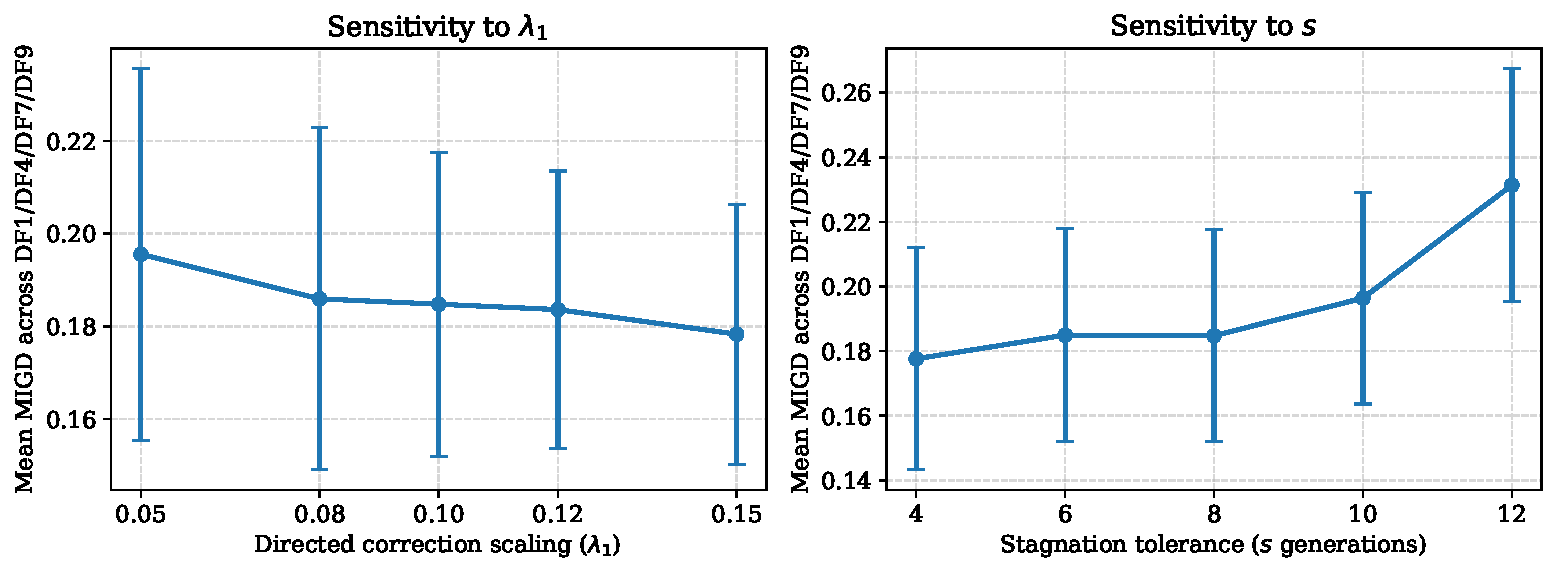
\includegraphics[width=\textwidth]{../experiments/results/sensitivity_analysis.pdf}
\caption{Multi-problem sensitivity analysis of the directed correction scaling $\lambda_1$ (left) and the stagnation tolerance $s$ (right). Points show aggregate mean MIGD over DF1, DF4, DF7, and DF9 under the moderate protocol; error bars show 95\% confidence intervals over the pooled sensitivity runs.}
\label{fig:sensitivity}
\end{figure}

\subsection{Ablation analysis}

\begin{table}[!t]
\centering
\caption{Average MIGD ranks for FITO component ablations across dynamic protocols. Lower is better.}
\label{tab:dynamic-ablation-ranks}
\resizebox{\textwidth}{!}{%
\begin{tabular}{lccccccc}
\toprule
Protocol & FITO & FITO-noLS & FITO-noRD & FITO-noPA & FITO-noPS & FITO+BR & FITO+MB \\
\midrule
fast\_t5\_n10 & \textbf{2.506} & 5.628 & 5.639 & 4.756 & \textbf{2.506} & 3.183 & 3.783 \\
moderate\_t10\_n10 & \textbf{2.350} & 6.433 & 4.994 & 4.267 & 3.583 & 3.100 & 3.272 \\
severe\_t10\_n20 & \textbf{2.694} & 6.489 & 4.328 & 4.122 & 3.744 & 3.500 & 3.122 \\
\midrule
Overall & \textbf{2.517} & 6.183 & 4.987 & 4.381 & 3.278 & 3.261 & 3.393 \\
\bottomrule
\end{tabular}
}
\end{table}


Table~\ref{tab:dynamic-ablation-ranks} clarifies which FITO mechanisms survive the broader protocol audit. Leader-support coordination and redeployment remain indispensable: FITO-noLS and FITO-noRD are the two weakest variants by a large margin. Predictive anchors are also helpful overall, although their effect is smaller and more problem-dependent. The critical revision concerns pit-stop restart. Under the expanded protocols, disabling pit-stop restart worsens 15 of the 27 protocol-problem cells, and the restart-enabled default is better on the moderate and severe \texttt{taut}=10 protocols while tying on the fast \texttt{taut}=5 protocol where the branch is inactive. The fixed-budget pit-stop probe shows the same direction, with FITO averaging rank 1.386 versus 1.614 for FITO-noPS. Boundary-risk scaling and anchor-leader blending remain unnecessary: FITO+BR and FITO+MB are still clearly behind the final default.

\subsection{Static sanity check}

Appendix~\ref{app:static} reports the static benchmark results under the same internal stagnation score and restart rule used in the dynamic default. FITO again attains the best mean HV and IGD on all five ZDT instances in the shipped appendix tables. The static ablation is consistent with, but does not independently prove, the usefulness of restart: FITO outperforms FITO-noSR on both ZDT4 metrics, while ZDT6 is effectively tied in HV and slightly favors FITO-noSR in IGD. The proper interpretation is therefore conservative. The static evidence shows that the dynamic default does not collapse on standard ZDT landscapes, but the paper's main claim still lives or dies on the dynamic protocols.

\subsection{Walk-forward portfolio suite}

This subsection should be read as a secondary walk-forward case study. It tests whether the dynamic-tracking behavior observed on synthetic DMOO benchmarks transfers to a noisy deployment setting, but it does not establish a general finance claim. The interpretation is intentionally conservative because the displayed MHV, MIGD, and deployment tables assign the best result to different algorithms and different universes. Table~\ref{tab:portfolio-scope} summarizes this deliberately limited reading before the detailed metric tables are reported.

\begin{table*}[!t]
\centering
\small
\caption{Conservative interpretation of the secondary walk-forward portfolio stress test.}
\label{tab:portfolio-scope}
\begin{tabular}{p{0.24\textwidth}p{0.32\textwidth}p{0.36\textwidth}}
\toprule
Evidence block & Observed winner pattern & Manuscript interpretation \\
\midrule
Technology universe (tech14), final wealth & FITO is strongest under the primary closest-to-utopia deployment rule. & Supports a limited claim that leader-motion redeployment can help when sectoral drift is coherent. \\
Broader market universe (market20), final wealth & NSGA-II is stronger than FITO. & Rejects any universal finance or investment-performance claim. \\
Frontier-transfer quality (MHV sensitivity counts) & MDDM-DMOEA is strongest in several settings. & Shows that deployment wealth and frontier-transfer quality do not identify the same winner. \\
Rule/cost sensitivity & Wealth winners are split across algorithms. & Positions the portfolio study as a stress test of boundary conditions, not as real-world validation. \\
\bottomrule
\end{tabular}
\end{table*}


\begin{table}[!t]
\centering
\small
\caption{Main-family out-of-sample normalized hypervolume (MHV) for the secondary walk-forward portfolio stress test. The table is generated from \texttt{asoc\_portfolio\_mhv\_summary.csv}; higher values are better, and both the 14-asset technology universe and 20-asset market universe are reported.}
\label{tab:portfolio-mhv}
\resizebox{\textwidth}{!}{%
\begin{tabular}{lccccccc}
\toprule
Universe & FITO & DNSGA-II-A & DNSGA-II-B & KGB-DMOEA & MDDM-DMOEA & NSGA-II & PPS-DMOEA \\
\midrule
tech14 (14 assets) & 0.4148 $\pm$ 0.0388 & 0.4149 $\pm$ 0.0169 & 0.3947 $\pm$ 0.0304 & 0.3482 $\pm$ 0.0112 & \textbf{0.4247 $\pm$ 0.0320} & 0.3760 $\pm$ 0.0236 & 0.3916 $\pm$ 0.0317 \\
market20 (20 assets) & 0.2393 $\pm$ 0.0177 & 0.2790 $\pm$ 0.0129 & 0.2506 $\pm$ 0.0148 & 0.2560 $\pm$ 0.0148 & \textbf{0.2858 $\pm$ 0.0154} & 0.2552 $\pm$ 0.0109 & 0.2479 $\pm$ 0.0152 \\
\bottomrule
\end{tabular}
}
\end{table}


\begin{table}[!t]
\centering
\small
\caption{Main-family out-of-sample mean inverted generational distance (MIGD) for the secondary walk-forward portfolio stress test. The table is generated from \texttt{asoc\_portfolio\_migd\_summary.csv}; lower values are better, and both the 14-asset technology universe and 20-asset market universe are reported.}
\label{tab:portfolio-migd}
\resizebox{\textwidth}{!}{%
\begin{tabular}{lccccccc}
\toprule
Universe & FITO & DNSGA-II-A & DNSGA-II-B & KGB-DMOEA & MDDM-DMOEA & NSGA-II & PPS-DMOEA \\
\midrule
tech14 (14 assets) & 0.0011 $\pm$ 0.0001 & 0.0011 $\pm$ 0.0001 & 0.0011 $\pm$ 0.0001 & 0.0013 $\pm$ 0.0001 & \textbf{0.0010 $\pm$ 0.0001} & 0.0012 $\pm$ 0.0001 & 0.0011 $\pm$ 0.0001 \\
market20 (20 assets) & 0.0011 $\pm$ 0.0000 & \textbf{0.0010 $\pm$ 0.0000} & 0.0011 $\pm$ 0.0000 & 0.0010 $\pm$ 0.0000 & 0.0010 $\pm$ 0.0000 & 0.0010 $\pm$ 0.0000 & 0.0011 $\pm$ 0.0000 \\
\bottomrule
\end{tabular}
}
\end{table}


Tables~\ref{tab:portfolio-mhv} and \ref{tab:portfolio-migd} are deliberately two-universe tables: rows report the 14-asset technology universe (tech14) and the 20-asset diversified market universe (market20), whereas columns report the seven competing algorithms. The portfolio evidence is therefore not a single-universe result. The application story is mixed rather than FITO-dominant. On the original technology universe, MDDM-DMOEA has the highest mean normalized HV (0.4247), while FITO (0.4148) and DNSGA-II-A (0.4149) are essentially tied behind it. The IGD view is also not a FITO win: MDDM-DMOEA gives the lowest mean IGD on tech14 (0.001041), followed by DNSGA-II-A (0.001062) and FITO (0.001082). On the broader market20 universe, MDDM-DMOEA again gives the highest mean normalized HV (0.2858), whereas DNSGA-II-A gives the lowest mean IGD (0.000992). FITO is weaker on both market20 frontier-transfer indicators, with mean normalized HV 0.2393 and mean IGD 0.001122. These values support the conservative interpretation that the portfolio suite exposes boundary conditions rather than a general financial advantage.

\begin{table}[!t]
\centering
\small
\caption{Main-family walk-forward deployment metrics for both portfolio universes under the closest-to-utopia selection rule at 10 bps. Values are generated from the flattened \texttt{asoc\_portfolio\_deployment\_summary.csv}; both universes and all seven ASOC algorithms are shown.}
\label{tab:portfolio-deployment}
\resizebox{\textwidth}{!}{%
\begin{tabular}{llcccc}
\toprule
Universe & Algorithm & Final wealth & Ann. return & Ann. vol. & Mean turnover \\
\midrule
tech14 (14 assets) & FITO & \textbf{41.618 $\pm$ 12.617} & 0.473 & 0.279 & 0.345 \\
tech14 (14 assets) & DNSGA-II-A & 34.609 $\pm$ 6.621 & 0.450 & 0.262 & 0.343 \\
tech14 (14 assets) & DNSGA-II-B & 31.140 $\pm$ 7.573 & 0.432 & 0.269 & 0.322 \\
tech14 (14 assets) & KGB-DMOEA & 21.728 $\pm$ 3.395 & 0.381 & 0.234 & 0.330 \\
tech14 (14 assets) & MDDM-DMOEA & 34.715 $\pm$ 10.177 & 0.446 & 0.282 & 0.370 \\
tech14 (14 assets) & NSGA-II & 24.832 $\pm$ 3.332 & 0.401 & 0.268 & 0.033 \\
tech14 (14 assets) & PPS-DMOEA & 27.783 $\pm$ 7.187 & 0.415 & 0.267 & 0.334 \\
\midrule
market20 (20 assets) & FITO & 5.744 $\pm$ 0.488 & 0.202 & 0.164 & 0.254 \\
market20 (20 assets) & DNSGA-II-A & 6.058 $\pm$ 0.447 & 0.208 & 0.163 & 0.290 \\
market20 (20 assets) & DNSGA-II-B & 5.520 $\pm$ 0.366 & 0.197 & 0.162 & 0.234 \\
market20 (20 assets) & KGB-DMOEA & 5.810 $\pm$ 0.405 & 0.203 & 0.158 & 0.309 \\
market20 (20 assets) & MDDM-DMOEA & 5.887 $\pm$ 0.454 & 0.205 & 0.166 & 0.280 \\
market20 (20 assets) & NSGA-II & \textbf{6.404 $\pm$ 0.489} & 0.216 & 0.162 & 0.054 \\
market20 (20 assets) & PPS-DMOEA & 5.570 $\pm$ 0.403 & 0.198 & 0.161 & 0.228 \\
\bottomrule
\end{tabular}
}
\end{table}


\begin{table}[!t]
\centering
\small
\caption{Deterministic deployment references for the secondary walk-forward portfolio stress test under the primary 10 bps cost setting. These references provide scale only and are not included in FITO-versus-DMOEA statistical tests.}
\label{tab:portfolio-benchmarks}
\resizebox{\textwidth}{!}{%
\begin{tabular}{llcccc}
\toprule
Universe & Reference & Final wealth & Ann. return & Ann. vol. & Mean turnover \\
\midrule
tech14 (14 assets) & EqualWeight & 7.987 & 0.244 & 0.237 & 0.000 \\
tech14 (14 assets) & RollingMinVar & 4.155 & 0.162 & 0.202 & 0.202 \\
\midrule
market20 (20 assets) & EqualWeight & 4.201 & 0.163 & 0.170 & 0.000 \\
market20 (20 assets) & RollingMinVar & 3.473 & 0.140 & 0.153 & 0.230 \\
\bottomrule
\end{tabular}
}
\end{table}


The deterministic EqualWeight and RollingMinVar references in Table~\ref{tab:portfolio-benchmarks} are included only as deployment baselines for scale; they are not evolutionary optimizers and are not part of the FITO-versus-DMOEA statistical tests.

The deployment view is more favorable to FITO on the technology universe than on the broader market universe. Table~\ref{tab:portfolio-deployment} is likewise block-partitioned by universe and restricted to the main family: the first block reports tech14, and the second block reports market20. The table includes all seven algorithms in both blocks. On tech14, FITO gives the highest mean final wealth (41.618 $\pm$ 12.617), followed by MDDM-DMOEA (34.715 $\pm$ 10.177) and DNSGA-II-A (34.609 $\pm$ 6.621). On market20, NSGA-II gives the highest mean final wealth (6.404 $\pm$ 0.489), while FITO gives 5.744 $\pm$ 0.488. The same table therefore prevents a one-sided reading: FITO is strongest in the coherent technology-universe deployment view, but NSGA-II is stronger on the broader market universe and MDDM-DMOEA leads the main MHV summaries in both universes. Across the displayed MHV, MIGD, and deployment tables, the winner pattern remains split rather than FITO-dominant. The correct reading is therefore not that FITO is a generally superior investment engine. The narrower reading is that FITO can be useful when the deployed universe has coherent sectoral drift, while diversified universes and frontier-transfer metrics can favor different optimizers.

This performance divergence highlights a critical boundary condition of the predictive redeployment mechanism, driven by \textit{topological fracture}. The 14-asset technology universe is highly correlated; when macroeconomic shocks occur, the true Pareto front shifts significantly in objective space, but its underlying geometric topology remains relatively stable. In such sector-specific environments, FITO's predictive anchors and change-triggered redeployment mechanism accurately capture the collective drift, successfully pulling the support pool toward the new front. Conversely, the 20-asset market universe contains weakly correlated and anti-correlated assets across diverse sectors. Environmental changes in this diverse universe cause the true Pareto front to jump erratically and alter its topological shape drastically. When the front topology fractures, recent leader motion becomes misleading. FITO's redeployment mechanism, which relies on this recent drift, suffers from negative transfer, steering the support pool into sub-optimal regions. Currently, FITO lacks a ``guard'' mechanism---such as a preliminary evaluation step to revert to a random fallback if the transferred individuals experience severe fitness degradation---to detect and reject this negative transfer. Furthermore, the increase in dimensionality (from $n=14$ to $n=20$) substantially increases the covering difficulty of the long-only allocation space, diluting the localized effectiveness of the pit-stop restart. In these highly volatile, topologically unstable environments, NSGA-II's globally dispersed population acts as a more robust fallback compared to FITO's tightly coordinated anchor dependencies.

\subsection{Implications}

The fixed-budget reframing changes the interpretation of the dynamic benchmark. The generation-matched suite shows that FITO is highly effective when the full response machinery is allowed to operate under a common generation horizon, but that suite also gives FITO more objective evaluations than several baselines. The approximately fixed-budget suite removes this confound and still ranks FITO first overall. The fair conclusion is therefore stronger and narrower: FITO's advantage is not solely an artifact of extra objective evaluations, because the method remains first under an approximately equalized evaluation budget; however, the advantage is not uniform across all landscapes. DF2 shows that recent leader-motion transfer can be harmful when environmental change reassigns the active decision coordinate. DF7 shows that smooth objective-front motion can still hide a changing nonlinear decision-space linkage. The walk-forward suite, by contrast, is only a secondary stress test. It does not support a universal finance claim: FITO is competitive and sometimes best, especially in the technology-universe deployment view, but MDDM-DMOEA leads the main MHV summaries in both universes, DNSGA-II-A leads market20 MIGD, and NSGA-II is stronger on the broader market universe for final wealth. These mixed outcomes are useful because they expose boundary conditions rather than because they validate FITO as a general portfolio optimizer.

\section{Threats to validity}
\label{sec:validity}

Eight limitations remain. First, the dynamic study now covers DF1--DF9 and three protocols, but it is still limited to the DF family available in the current \texttt{pymoo} environment rather than a broader reproduced benchmark universe. Second, the primary fixed-budget study changes population size to normalize evaluations; this is a reasonable budget-control device for fairness-controlled evaluation, but it is not the same experimental question as equal-population benchmarking. Third, the fixed-budget population-size calibration uses a DF1, seed-0 pilot for each algorithm--protocol pair. This choice keeps the calibration lightweight and avoids tuning on all final outcomes, but a stronger future protocol would calibrate on several representative pilot problems, for example DF1, DF4, and DF7, and then freeze the resulting average population sizes before the full evaluation. The realized min--mean--max budget table is included to make the approximation auditable. Fourth, the component study is one-at-a-time rather than factorial, so interactions among pit-stop restart, redeployment, and predictive anchors are not yet fully resolved. Fifth, the baseline selection is restricted to algorithms with reproducible, open-source implementations. While the related-work section now covers recent 2023--2026 prediction, transfer-learning, adaptive-response, restart, and benchmark-design studies, reimplementing highly complex methods from scratch can introduce severe implementation bias. This risk is mitigated by including reproducible representatives of the major response families and by integrating an open-source KDE-based surrogate of the 2024 MDDM framework. Nevertheless, future comparisons against natively open-sourced implementations of newer methods such as HRS-DMOA, MOEA/D-HSS, DSDRS, RSAS, TMKT, EHEL, and generalized 2026 benchmark suites would further strengthen the empirical scope. Sixth, the DF2/DF7 failure-mode explanation combines observed performance patterns with benchmark formula inspection; it is a mechanistic interpretation rather than a separate causal ablation that directly switches coordinate-role and linkage dynamics on and off. Seventh, the walk-forward portfolio section is a secondary application stress test rather than a real-world validation study. It uses only two equity universes, one 252/63 walk-forward schedule, three decision rules, and three cost levels; the mixed results are insufficient for any general finance or investment-performance claim. Eighth, the portfolio protocol still contains finance-specific simplifications: the fixed asset universes may embed survivorship or selection bias; the 2013-05-23--2022-11-22 holdout schedule may favor particular market regimes; the proportional transaction-cost model omits liquidity, market impact, bid--ask spread dynamics, taxes, borrowing, and slippage; and the long-only frontier excludes short-selling, leverage, and explicit cash allocation. These restrictions make the portfolio suite useful as a stress test of dynamic tracking behavior, but not as an investment validation study.

\section{Conclusion}
\label{sec:conclusion}

This paper presents a reproducible dynamic multi-objective evolutionary optimizer mathematically grounded as a DE-inspired bipartite team-guided evolutionary architecture with asymmetric elitism and local random restart, conceptually inspired by Formula 1 team coordination principles. Under the expanded DF1--DF9 benchmark suite with three change protocols, FITO achieves the best primary fixed-budget overall average MIGD rank (1.898) when objective-evaluation counts are approximately equalized around 8000 evaluations per run. The generation-matched result remains consistent, with an overall diagnostic rank of 1.554, but it is not used as the primary fairness-controlled evidence because FITO performs more objective evaluations than several baselines under the common-generation protocol. The component analysis gives a clearer mechanism story: leader-support coordination, redeployment, predictive anchors, and pit-stop restart are useful under the broader protocols, whereas boundary-risk scaling and anchor-leader blending should be excluded from the default. The default FITO obtains an ablation average rank of 2.517, compared with 3.278 without pit-stop restart, and the separate fixed-budget pit-stop probe gives 1.386 versus 1.614. The static ZDT study remains a secondary sanity check, not the primary claim. The walk-forward portfolio suite deliberately narrows the application narrative: it is a secondary stress test, not a real-world validation study. FITO is strongest only in the 14-asset technology-universe deployment final-wealth view, while MDDM-DMOEA is stronger in the main MHV summaries for both universes and NSGA-II is stronger on the broader 20-asset universe for final wealth. Consequently, FITO should be interpreted as a competitive budget-aware dynamic tracking framework rather than a universally dominant optimizer or a generally superior portfolio method. The DF2 and DF7 failure-mode analysis narrows this interpretation further: leader-motion transfer is useful when the decision-space manifold moves coherently, but it can become negative transfer when active coordinate roles switch or nonlinear linkages reverse quickly. While highly volatile, high-dimensional topologies remain challenging, the rapid recovery mechanisms are useful for domains characterized by recurring or topologically stable environmental drift. Because exact hypervolume computation becomes rapidly more expensive as the number of objectives increases, future many-objective extensions should substitute the stagnation trigger with cheaper alternatives such as the R2 indicator or generational-distance metrics. Future work will also integrate localized topology estimation, transfer-quality probes, and adaptive restart radii to detect and alleviate negative transfer in diverse, large-scale systems.

\section*{Data availability}

The implementation scripts, cached market data, generated raw/result artifacts, manuscript source, and compiled manuscript snapshot are available in the public repository \url{https://github.com/ErcanErkalkan/Formula_Inspired_Team_Based_Optimization_for_Decision_Making_and_Strategy_in_Dynamic_Systems}.

The repository includes a reviewer-oriented \path{README.md}, pinned Python dependencies in \path{requirements.txt}, a Conda wrapper in \path{environment.yml}, Windows and Linux/macOS reproduction entry points through \path{reproduce_all.ps1} and \path{reproduce_all.sh}, a \path{Makefile} with separate \path{smoke}, \path{tables}, and \path{full} targets, and a \path{SHA256SUMS.txt} manifest generated by \path{scripts/generate_checksums.py}. The command \path{python experiments/smoke_test.py} performs a quick reproducibility smoke test. The commands \path{bash reproduce_all.sh --tables-only} and \path{.\reproduce_all.ps1 -TablesOnly} rebuild the dynamic and portfolio report tables plus the manuscript from existing raw artifacts; precomputed static ZDT appendix tables are kept as shipped unless \path{run_benchmarks.py} is executed. The commands \path{bash reproduce_all.sh} and \path{.\reproduce_all.ps1} rerun the full experimental pipeline.

The primary fixed-budget dynamic benchmark outputs are stored under \path{experiments/results/asoc_dynamic_budget_*}; auxiliary generation-matched diagnostic outputs are stored under \path{experiments/results/asoc_dynamic_eval_budget*} and \path{experiments/results/asoc_dynamic_protocol_ranks.tex}; and the secondary walk-forward portfolio stress-test outputs are stored under \path{experiments/results/asoc_portfolio_*}.

\section*{Funding}

This research received no specific grant from funding agencies in the public, commercial, or not-for-profit sectors.

\section*{Declaration of generative AI and AI-assisted technologies in the writing process}

During the preparation of this work, the author used AI-assisted tools for language editing, code inspection, and consistency checks. All technical decisions, experimental redesign, verification, and final manuscript content were reviewed and approved by the author, who takes full responsibility for the submitted work.

\section*{Declaration of competing interest}

The author declares no known competing financial interests or personal relationships that could have appeared to influence the work reported in this paper.

\bibliographystyle{elsarticle-num}
\bibliography{asoc_refs}

\clearpage
\appendix

\section{Dynamic protocol tables}
\label{app:dynamic}

Tables~\ref{tab:dynamic-fast_t5_n10}--\ref{tab:dynamic-severe_t10_n20} report auxiliary generation-matched protocol results obtained with a common population size of 100. They are included only as diagnostic protocol-level detail. Their MIGD values should not be compared directly with the primary fixed-budget failure-mode values in the main text, because the fixed-budget study uses protocol-specific population calibration to approximately equalize objective-evaluation counts. Tables~\ref{tab:dynamic-eval-budget} and~\ref{tab:dynamic-fixed-budget} make this distinction explicit by reporting nominal evaluation counts, separate response-refresh counts, total objective-call means, and the realized primary fixed-budget audit, respectively.

\begin{table}[H]
\centering
\caption{Auxiliary generation-matched protocol results for the fast taut=5, nt=10 dynamic protocol. These diagnostic values are not the primary fixed-budget values discussed in the main text.}
\label{tab:dynamic-fast_t5_n10}
\resizebox{\textwidth}{!}{%
\begin{tabular}{lccccccc}
\toprule
Problem & FITO & DNSGA-II-A & DNSGA-II-B & KGB-DMOEA & MDDM-DMOEA & NSGA-II & PPS-DMOEA \\
\midrule
DF1 & 0.1161 $\pm$ 0.0196 & 0.2212 $\pm$ 0.0251 & 0.5957 $\pm$ 0.0755 & 0.2463 $\pm$ 0.0391 & 0.5153 $\pm$ 0.0744 & \textbf{0.1147 $\pm$ 0.0226} & 0.5571 $\pm$ 0.0527 \\
DF2 & 0.2494 $\pm$ 0.0189 & 0.1458 $\pm$ 0.0160 & 0.4426 $\pm$ 0.0633 & 0.1860 $\pm$ 0.0252 & 0.3863 $\pm$ 0.0450 & \textbf{0.1028 $\pm$ 0.0179} & 0.4691 $\pm$ 0.0710 \\
DF3 & \textbf{0.5382 $\pm$ 0.1087} & 0.7794 $\pm$ 0.0744 & 0.7387 $\pm$ 0.0697 & 0.7137 $\pm$ 0.0849 & 0.6730 $\pm$ 0.1120 & 0.6011 $\pm$ 0.1355 & 0.7147 $\pm$ 0.0956 \\
DF4 & \textbf{0.3232 $\pm$ 0.0490} & 0.9312 $\pm$ 0.1316 & 0.8843 $\pm$ 0.1377 & 1.0650 $\pm$ 0.2424 & 0.8093 $\pm$ 0.1161 & 0.9510 $\pm$ 0.1511 & 0.8631 $\pm$ 0.1407 \\
DF5 & \textbf{0.0671 $\pm$ 0.0076} & 0.3063 $\pm$ 0.0357 & 0.2818 $\pm$ 0.0369 & 0.3305 $\pm$ 0.0491 & 0.2360 $\pm$ 0.0286 & 0.2249 $\pm$ 0.0428 & 0.2835 $\pm$ 0.0270 \\
DF6 & \textbf{5.0920 $\pm$ 0.5949} & 9.1439 $\pm$ 0.8813 & 12.3513 $\pm$ 1.9642 & 9.4009 $\pm$ 1.1145 & 9.1144 $\pm$ 0.6079 & 9.4975 $\pm$ 1.8682 & 11.3229 $\pm$ 1.0108 \\
DF7 & 0.2372 $\pm$ 0.0702 & 0.3037 $\pm$ 0.0409 & 0.2862 $\pm$ 0.0416 & 0.3409 $\pm$ 0.0302 & 0.1873 $\pm$ 0.0391 & \textbf{0.1700 $\pm$ 0.0357} & 0.2762 $\pm$ 0.0420 \\
DF8 & \textbf{0.0825 $\pm$ 0.0049} & 0.1375 $\pm$ 0.0155 & 0.1247 $\pm$ 0.0193 & 0.2326 $\pm$ 0.0295 & 0.1132 $\pm$ 0.0078 & 0.1427 $\pm$ 0.0125 & 0.1182 $\pm$ 0.0127 \\
DF9 & \textbf{0.3427 $\pm$ 0.0484} & 0.6388 $\pm$ 0.0432 & 0.7981 $\pm$ 0.1773 & 1.1237 $\pm$ 0.2255 & 0.6167 $\pm$ 0.0984 & 0.4801 $\pm$ 0.0781 & 0.7313 $\pm$ 0.1302 \\
\bottomrule
\end{tabular}
}
\end{table}


\begin{table}[H]
\centering
\caption{Auxiliary generation-matched protocol results for the moderate taut=10, nt=10 dynamic protocol. These diagnostic values are not the primary fixed-budget values discussed in the main text.}
\label{tab:dynamic-moderate_t10_n10}
\resizebox{\textwidth}{!}{%
\begin{tabular}{lccccccc}
\toprule
Problem & FITO & DNSGA-II-A & DNSGA-II-B & KGB-DMOEA & MDDM-DMOEA & NSGA-II & PPS-DMOEA \\
\midrule
DF1 & \textbf{0.0899 $\pm$ 0.0152} & 0.1966 $\pm$ 0.0184 & 0.2843 $\pm$ 0.0326 & 0.1865 $\pm$ 0.0210 & 0.2598 $\pm$ 0.0230 & 0.1085 $\pm$ 0.0183 & 0.2818 $\pm$ 0.0285 \\
DF2 & 0.1840 $\pm$ 0.0203 & 0.1341 $\pm$ 0.0140 & 0.3083 $\pm$ 0.0293 & 0.1383 $\pm$ 0.0203 & 0.2919 $\pm$ 0.0329 & \textbf{0.1164 $\pm$ 0.0364} & 0.3062 $\pm$ 0.0339 \\
DF3 & \textbf{0.2992 $\pm$ 0.1215} & 0.6550 $\pm$ 0.1192 & 0.6401 $\pm$ 0.1243 & 0.5590 $\pm$ 0.0564 & 0.6085 $\pm$ 0.1316 & 0.5372 $\pm$ 0.1154 & 0.6175 $\pm$ 0.1160 \\
DF4 & \textbf{0.3449 $\pm$ 0.0491} & 0.9749 $\pm$ 0.1605 & 0.9637 $\pm$ 0.1520 & 0.9577 $\pm$ 0.1448 & 0.8962 $\pm$ 0.1526 & 0.9254 $\pm$ 0.1887 & 0.9152 $\pm$ 0.1579 \\
DF5 & \textbf{0.0617 $\pm$ 0.0058} & 0.2064 $\pm$ 0.0194 & 0.1900 $\pm$ 0.0159 & 0.1948 $\pm$ 0.0125 & 0.1827 $\pm$ 0.0173 & 0.1517 $\pm$ 0.0185 & 0.1893 $\pm$ 0.0130 \\
DF6 & \textbf{6.4833 $\pm$ 1.8608} & 11.2216 $\pm$ 0.8364 & 14.1694 $\pm$ 2.6060 & 10.9902 $\pm$ 1.1362 & 11.1402 $\pm$ 1.0068 & 8.4695 $\pm$ 1.7302 & 12.5270 $\pm$ 1.3444 \\
DF7 & \textbf{0.1259 $\pm$ 0.0425} & 0.3077 $\pm$ 0.0772 & 0.2931 $\pm$ 0.0740 & 0.3269 $\pm$ 0.0649 & 0.2205 $\pm$ 0.1004 & 0.1947 $\pm$ 0.0345 & 0.2799 $\pm$ 0.0683 \\
DF8 & \textbf{0.0619 $\pm$ 0.0039} & 0.1039 $\pm$ 0.0092 & 0.1012 $\pm$ 0.0100 & 0.1647 $\pm$ 0.0230 & 0.0971 $\pm$ 0.0071 & 0.1470 $\pm$ 0.0078 & 0.0991 $\pm$ 0.0066 \\
DF9 & \textbf{0.1833 $\pm$ 0.0299} & 0.4679 $\pm$ 0.0633 & 0.4894 $\pm$ 0.0570 & 0.6527 $\pm$ 0.1495 & 0.3776 $\pm$ 0.0469 & 0.3726 $\pm$ 0.0651 & 0.4530 $\pm$ 0.0596 \\
\bottomrule
\end{tabular}
}
\end{table}


\begin{table}[!t]
\centering
\caption{MIGD results on the severe t10 n20 dynamic protocol over 20 independent runs.}
\label{tab:dynamic-severe_t10_n20}
\resizebox{\textwidth}{!}{%
\begin{tabular}{lccccccc}
\toprule
Problem & FITO & DNSGA-II-A & DNSGA-II-B & KGB-DMOEA & MDDM-DMOEA & NSGA-II & PPS-DMOEA \\
\midrule
DF1 & \textbf{0.0722 $\pm$ 0.0135} & 0.1357 $\pm$ 0.0167 & 0.1312 $\pm$ 0.0160 & 0.1565 $\pm$ 0.0199 & 0.1315 $\pm$ 0.0192 & 0.1071 $\pm$ 0.0196 & 0.1325 $\pm$ 0.0178 \\
DF2 & 0.1688 $\pm$ 0.0205 & 0.1133 $\pm$ 0.0200 & 0.2294 $\pm$ 0.0204 & 0.1231 $\pm$ 0.0228 & 0.2302 $\pm$ 0.0243 & \textbf{0.0750 $\pm$ 0.0145} & 0.2362 $\pm$ 0.0223 \\
DF3 & \textbf{0.2020 $\pm$ 0.0722} & 0.5152 $\pm$ 0.1309 & 0.5002 $\pm$ 0.1293 & 0.4339 $\pm$ 0.0588 & 0.4837 $\pm$ 0.1036 & 0.4703 $\pm$ 0.0903 & 0.5010 $\pm$ 0.1061 \\
DF4 & \textbf{0.2967 $\pm$ 0.0501} & 0.9318 $\pm$ 0.1606 & 0.9211 $\pm$ 0.1609 & 0.9460 $\pm$ 0.1578 & 0.8598 $\pm$ 0.1620 & 0.9113 $\pm$ 0.1787 & 0.8684 $\pm$ 0.1554 \\
DF5 & \textbf{0.0477 $\pm$ 0.0046} & 0.1369 $\pm$ 0.0152 & 0.1312 $\pm$ 0.0156 & 0.1720 $\pm$ 0.0219 & 0.1268 $\pm$ 0.0123 & 0.1230 $\pm$ 0.0151 & 0.1290 $\pm$ 0.0127 \\
DF6 & 6.2253 $\pm$ 3.2956 & 8.1675 $\pm$ 1.0464 & 8.4457 $\pm$ 1.3642 & 10.2178 $\pm$ 1.2439 & 7.9000 $\pm$ 1.5033 & \textbf{5.9840 $\pm$ 1.3529} & 7.8197 $\pm$ 1.2361 \\
DF7 & \textbf{0.1295 $\pm$ 0.0573} & 0.3276 $\pm$ 0.0794 & 0.3107 $\pm$ 0.0762 & 0.3506 $\pm$ 0.0713 & 0.2187 $\pm$ 0.0964 & 0.2304 $\pm$ 0.0488 & 0.2831 $\pm$ 0.0733 \\
DF8 & \textbf{0.0309 $\pm$ 0.0029} & 0.0787 $\pm$ 0.0089 & 0.0741 $\pm$ 0.0077 & 0.1147 $\pm$ 0.0127 & 0.0713 $\pm$ 0.0068 & 0.0759 $\pm$ 0.0076 & 0.0723 $\pm$ 0.0065 \\
DF9 & \textbf{0.1210 $\pm$ 0.0180} & 0.3415 $\pm$ 0.0540 & 0.3495 $\pm$ 0.0599 & 0.4110 $\pm$ 0.0503 & 0.2685 $\pm$ 0.0350 & 0.2975 $\pm$ 0.0453 & 0.3100 $\pm$ 0.0455 \\
\bottomrule
\end{tabular}
}
\end{table}


\begin{table}[!t]
\centering
\caption{Dynamic generation-matched evaluation and runtime summary.}
\label{tab:dynamic-eval-budget}
\resizebox{\textwidth}{!}{%
\begin{tabular}{llccc}
\toprule
Protocol & Algorithm & Mean evals & Mean pop & Mean runtime (s) \\
\midrule
fast\_t5\_n10 & FITO & 12196.0 & 100.0 & 0.984 \\
fast\_t5\_n10 & DNSGA-II-A & 7790.0 & 100.0 & 1.082 \\
fast\_t5\_n10 & DNSGA-II-B & 7790.0 & 100.0 & 1.075 \\
fast\_t5\_n10 & KGB-DMOEA & 7943.0 & 100.0 & 3.470 \\
fast\_t5\_n10 & MDDM-DMOEA & 6000.0 & 100.0 & 1.032 \\
fast\_t5\_n10 & NSGA-II & 6000.0 & 100.0 & 0.937 \\
fast\_t5\_n10 & PPS-DMOEA & 6000.0 & 100.0 & 1.035 \\
\midrule
moderate\_t10\_n10 & FITO & 12207.9 & 100.0 & 0.964 \\
moderate\_t10\_n10 & DNSGA-II-A & 7190.0 & 100.0 & 1.080 \\
moderate\_t10\_n10 & DNSGA-II-B & 7190.0 & 100.0 & 1.081 \\
moderate\_t10\_n10 & KGB-DMOEA & 7266.5 & 100.0 & 6.180 \\
moderate\_t10\_n10 & MDDM-DMOEA & 6000.0 & 100.0 & 1.020 \\
moderate\_t10\_n10 & NSGA-II & 6000.0 & 100.0 & 0.978 \\
moderate\_t10\_n10 & PPS-DMOEA & 6000.0 & 100.0 & 1.021 \\
\midrule
severe\_t10\_n20 & FITO & 12208.1 & 100.0 & 0.953 \\
severe\_t10\_n20 & DNSGA-II-A & 7190.0 & 100.0 & 1.062 \\
severe\_t10\_n20 & DNSGA-II-B & 7190.0 & 100.0 & 1.052 \\
severe\_t10\_n20 & KGB-DMOEA & 7266.4 & 100.0 & 8.037 \\
severe\_t10\_n20 & MDDM-DMOEA & 6000.0 & 100.0 & 1.007 \\
severe\_t10\_n20 & NSGA-II & 6000.0 & 100.0 & 0.945 \\
severe\_t10\_n20 & PPS-DMOEA & 6000.0 & 100.0 & 0.993 \\
\bottomrule
\end{tabular}
}
\end{table}


\begin{table}[!t]
\centering
\caption{Primary fixed-budget dynamic audit. The calibration equalizes the nominal optimizer budget; response-refresh evaluations for predictive baselines are reported separately, and total objective calls are shown explicitly.}
\label{tab:dynamic-fixed-budget}
\resizebox{\textwidth}{!}{%
\begin{tabular}{llccccc}
\toprule
Protocol & Algorithm & Nom. eval. & Resp. eval. & Total calls & Pop. mean & Pop. range \\
\midrule
fast\_t5\_n10 & FITO & 8046.0 & 0.0 & 8046.0 & 66.0 & 66--66 \\
fast\_t5\_n10 & DNSGA-II-A & 8065.0 & 0.0 & 8065.0 & 103.0 & 103--103 \\
fast\_t5\_n10 & DNSGA-II-B & 8065.0 & 0.0 & 8065.0 & 103.0 & 103--103 \\
fast\_t5\_n10 & KGB-DMOEA & 8073.9 & 0.0 & 8073.9 & 101.0 & 101--101 \\
fast\_t5\_n10 & MDDM-DMOEA & 7980.0 & 1596.0 & 9576.0 & 133.0 & 133--133 \\
fast\_t5\_n10 & NSGA-II & 7980.0 & 0.0 & 7980.0 & 133.0 & 133--133 \\
fast\_t5\_n10 & PPS-DMOEA & 7980.0 & 1596.0 & 9576.0 & 133.0 & 133--133 \\
\midrule
moderate\_t10\_n10 & FITO & 8054.8 & 0.0 & 8054.8 & 66.0 & 66--66 \\
moderate\_t10\_n10 & DNSGA-II-A & 8034.0 & 0.0 & 8034.0 & 111.0 & 111--111 \\
moderate\_t10\_n10 & DNSGA-II-B & 8034.0 & 0.0 & 8034.0 & 111.0 & 111--111 \\
moderate\_t10\_n10 & KGB-DMOEA & 7985.5 & 0.0 & 7985.5 & 110.0 & 110--110 \\
moderate\_t10\_n10 & MDDM-DMOEA & 7980.0 & 798.0 & 8778.0 & 133.0 & 133--133 \\
moderate\_t10\_n10 & NSGA-II & 7980.0 & 0.0 & 7980.0 & 133.0 & 133--133 \\
moderate\_t10\_n10 & PPS-DMOEA & 7980.0 & 798.0 & 8778.0 & 133.0 & 133--133 \\
\midrule
severe\_t10\_n20 & FITO & 8054.5 & 0.0 & 8054.5 & 66.0 & 66--66 \\
severe\_t10\_n20 & DNSGA-II-A & 8034.0 & 0.0 & 8034.0 & 111.0 & 111--111 \\
severe\_t10\_n20 & DNSGA-II-B & 8034.0 & 0.0 & 8034.0 & 111.0 & 111--111 \\
severe\_t10\_n20 & KGB-DMOEA & 7985.5 & 0.0 & 7985.5 & 110.0 & 110--110 \\
severe\_t10\_n20 & MDDM-DMOEA & 7980.0 & 798.0 & 8778.0 & 133.0 & 133--133 \\
severe\_t10\_n20 & NSGA-II & 7980.0 & 0.0 & 7980.0 & 133.0 & 133--133 \\
severe\_t10\_n20 & PPS-DMOEA & 7980.0 & 798.0 & 8778.0 & 133.0 & 133--133 \\
\bottomrule
\end{tabular}
}
\end{table}

\FloatBarrier
\clearpage

\section{Static benchmark and ablation tables}
\label{app:static}

\begin{table}[H]
\centering
\caption{Hypervolume results over 20 independent runs.}
\label{tab:hv}
\resizebox{\textwidth}{!}{%
\begin{tabular}{lcccc}
\toprule
Problem & FITO & NSGA-II & MOEA/D & RVEA \\
\midrule
ZDT1 & \textbf{0.8696 $\pm$ 0.0003} & 0.8672 $\pm$ 0.0005 & 0.8612 $\pm$ 0.0114 & 0.8209 $\pm$ 0.0070 \\
ZDT2 & \textbf{0.5366 $\pm$ 0.0005} & 0.5323 $\pm$ 0.0013 & 0.5046 $\pm$ 0.0500 & 0.4550 $\pm$ 0.0101 \\
ZDT3 & \textbf{1.3236 $\pm$ 0.0185} & 1.3197 $\pm$ 0.0183 & 1.3181 $\pm$ 0.0185 & 1.2001 $\pm$ 0.0228 \\
ZDT4 & \textbf{0.8699 $\pm$ 0.0008} & 0.8658 $\pm$ 0.0029 & 0.8574 $\pm$ 0.0077 & 0.7954 $\pm$ 0.0484 \\
ZDT6 & \textbf{0.5034 $\pm$ 0.0003} & 0.4701 $\pm$ 0.0037 & 0.4953 $\pm$ 0.0016 & 0.3004 $\pm$ 0.0253 \\
\bottomrule
\end{tabular}
}
\end{table}


\begin{table}[!t]
\centering
\caption{IGD results over 20 independent runs.}
\label{tab:igd}
\resizebox{\textwidth}{!}{%
\begin{tabular}{lcccc}
\toprule
Problem & FITO & NSGA-II & MOEA/D & RVEA \\
\midrule
ZDT1 & \textbf{0.0049 $\pm$ 0.0003} & 0.0055 $\pm$ 0.0003 & 0.0125 $\pm$ 0.0139 & 0.0325 $\pm$ 0.0043 \\
ZDT2 & \textbf{0.0050 $\pm$ 0.0006} & 0.0061 $\pm$ 0.0006 & 0.0249 $\pm$ 0.0399 & 0.0482 $\pm$ 0.0053 \\
ZDT3 & \textbf{0.0078 $\pm$ 0.0124} & 0.0084 $\pm$ 0.0124 & 0.0127 $\pm$ 0.0124 & 0.0532 $\pm$ 0.0108 \\
ZDT4 & \textbf{0.0046 $\pm$ 0.0004} & 0.0062 $\pm$ 0.0014 & 0.0126 $\pm$ 0.0094 & 0.0889 $\pm$ 0.0721 \\
ZDT6 & \textbf{0.0039 $\pm$ 0.0003} & 0.0250 $\pm$ 0.0026 & 0.0068 $\pm$ 0.0010 & 0.1500 $\pm$ 0.0198 \\
\bottomrule
\end{tabular}
}
\end{table}


\begin{table}[!t]
\centering
\caption{Static sanity check for selected FITO variants. FITO is the final dynamic default; FITO-noSR disables the stagnation restart for sensitivity analysis.}
\label{tab:ablation}
\resizebox{\textwidth}{!}{%
\begin{tabular}{llcccc}
\toprule
Problem & Metric & FITO & FITO+BR & FITO-noSR & FITO-noLS \\
\midrule
ZDT4 & HV & \textbf{0.86994 $\pm$ 0.00079} & 0.85897 $\pm$ 0.04958 & 0.86643 $\pm$ 0.00344 & 0.86491 $\pm$ 0.00264 \\
ZDT4 & IGD & \textbf{0.00463 $\pm$ 0.00038} & 0.01163 $\pm$ 0.03160 & 0.00604 $\pm$ 0.00171 & 0.00668 $\pm$ 0.00135 \\
ZDT6 & HV & \textbf{0.50342 $\pm$ 0.00028} & 0.50329 $\pm$ 0.00039 & 0.50338 $\pm$ 0.00033 & 0.48017 $\pm$ 0.00792 \\
ZDT6 & IGD & 0.00390 $\pm$ 0.00026 & 0.00394 $\pm$ 0.00039 & \textbf{0.00388 $\pm$ 0.00026} & 0.01797 $\pm$ 0.00516 \\
\bottomrule
\end{tabular}
}
\end{table}

\FloatBarrier

\end{document}
